\documentclass[10pt,journal,compsoc]{IEEEtran}

\usepackage[nocompress]{cite}
\usepackage{amsmath,amsfonts}
\usepackage{algorithmic}
\usepackage{algorithm}
\usepackage{array}
\usepackage[caption=false,font=footnotesize,labelfont=sf,textfont=sf]{subfig}
\usepackage{url}
\usepackage{textcomp}
\usepackage{stfloats}
\usepackage{verbatim}
\usepackage{graphicx}
\usepackage{cite}
%\usepackage{hyperref}
\usepackage{xspace}
\usepackage{color}
\usepackage{multirow}
\usepackage{multicol}
\usepackage{tabularx}
\usepackage{bigstrut}
\usepackage{booktabs}
\usepackage{bbding}
%\usepackage[nomarkers]{endfloat}

\let\MYoriglatexcaption\caption
\renewcommand{\caption}[2][\relax]{\MYoriglatexcaption[#2]{#2}}

\hyphenation{op-tical net-works semi-conduc-tor}

\newcommand{\sys}{I$^2$RNN\xspace}
\newcommand{\papertitle}{\sys: An Incremental and Interpretable Recurrent Neural Network for Encrypted Traffic Classification}
\newcommand{\etal}{et al.\xspace}
\newcommand{\ie}{i.e.,\xspace}
\newcommand{\eg}{e.g.,\xspace}
\newcommand{\todo}[1]{\textcolor{yellow}{TODO: #1}}
\newcommand{\first}{\textsf{(i)}\xspace}
\newcommand{\second}{\textsf{(ii)}\xspace}
\newcommand{\third}{\textsf{(iii)}\xspace}
\newcommand{\forth}{\textsf{(iv)}\xspace}
\newcommand{\five}{\textsf{(v)}\xspace}

\begin{document}

\title{\papertitle}

\author{Zhuoxue~Song,~%~\IEEEmembership{Member,~IEEE,
	     Ziming~Zhao,~%~\IEEEmembership{Fellow,~OSA,}
            Fan~Zhang\textsuperscript{\Envelope},~\IEEEmembership{Member,~IEEE},~
	     Gang~Xiong,~\\%~\IEEEmembership{Member,~IEEE},~\\%\IEEEmembership{Member,~IEEE},~\\
            Guang~Cheng,~\IEEEmembership{Member,~IEEE},~%\IEEEmembership{Member,~IEEE},~
            Xinjie~Zhao,~
            and~Shize~Guo\textcolor{white}{\textsuperscript{\Envelope}}% <-this % stops a space

\IEEEcompsocitemizethanks{\IEEEcompsocthanksitem Zhuoxue Song, Ziming Zhao, Xinjie Zhao, and Shize Guo are with the College of Computer Science and Technology, Zhejiang University, Hangzhou 310027, China. E-mail: \{songzhuoxue, zhaoziming\}@zju.edu.cn.%\protect\\
\IEEEcompsocthanksitem Fan Zhang is with the College of Computer Science and Technology, Zhejiang University, Hangzhou 310027, with ZJU-Hangzhou Global Scientific and Technological Innovation Center, Hangzhou 311200, with the Key Laboratory of Blockchain and Cyberspace Governance of Zhejiang Province, with Jiaxing Research Institute, Zhejiang University, Jiaxing 314000, and also with Zhengzhou Xinda Institute of Advanced Technology, Zhengzhou 450001, China. E-mail: fanzhang@zju.edu.cn.%\protect\\
\IEEEcompsocthanksitem Gang Xiong is with the Institute of Information Engineering, Chinese Academy of Sciences, Beijing 100190, China. E-mail: xionggang@iie.ac.cn.%\protect\\
\IEEEcompsocthanksitem Guang Cheng is with the School of Cyber Science and Engineering, Southeast University, Nanjing 211189, China. E-mail: chengguang@seu.edu.cn.%\protect\\
% note need leading \protect in front of \\ to get a newline within \thanks as
% \\ is fragile and will error, could use \hfil\break instead.
%\IEEEcompsocthanksitem J. Doe and J. Doe are with Anonymous University.
}% <-this % stops an unwanted space

\thanks{
Manuscript received 17 Feb. 2022; revised 10 Nov. 2022. (Corresponding author: Fan Zhang.)}
}

% The paper headers
\markboth{IEEE TRANSACTIONS ON DEPENDABLE AND SECURE COMPUTING, VOL. 19, NO. 1, JANUARY/FEBRUARY 2022}%
{Zhuoxue Song \MakeLowercase{\textit{et al.}}: \papertitle}

% use for special paper notices
%\IEEEspecialpapernotice{(Invited Paper)}

\IEEEtitleabstractindextext{
\begin{abstract}
Traffic classification occupies a significant role in cybersecurity and network management. 
The widespread of encryption transmission protocols such as SSL/TLS has led to the dominance of deep learning based approaches.
In cybersecurity, strong adversaries often complicate their strategies by constantly developing emerging attacks. 
Meanwhile, security practitioners desire to grasp the reasons for inference results. 
However, existing deep learning approaches lack efficient adaptation for incremental traffic types and often have less interpretability. 
In this paper, we propose \sys, an Incremental and Interpretable Recurrent Neural Network for encrypted traffic classification.  
The \sys proposes a novel propagation process to extract the sequence fingerprints from sessions with local robustness. 
Meanwhile, this proposal provides interpretability including time-series feature attribution and inter-class similarity portrait. 
Moreover, we design \sys in an incremental manner to adapt to emerging traffic types. 
The \sys only needs to train an additional set of parameters for the newly added traffic type rather than retraining the whole model with the entire dataset.  
Extensive experimental results show that our \sys can achieve remarkable performance in traffic classification, incremental learning, and model interpretability. 
Compared with other local interpretability methods, our \sys exhibits excellent stability, robustness, and effectiveness in the interpretation of network traffic data.
\end{abstract}
\begin{IEEEkeywords}
Encrypted traffic classification,  incremental learning,  interpretability, recurrent neural network
\end{IEEEkeywords}
}

\maketitle

\IEEEdisplaynontitleabstractindextext

\IEEEpeerreviewmaketitle

\IEEEraisesectionheading{\section{Introduction}\label{sec:Introduction}}

% The very first letter is a 2 line initial drop letter followed
% by the rest of the first word in caps (small caps for compsoc).
% 
% form to use if the first word consists of a single letter:
% \IEEEPARstart{A}{demo} file is ....
% 
% form to use if you need the single drop letter followed by
% normal text (unknown if ever used by the IEEE):
% \IEEEPARstart{A}{}demo file is ....
% 
% Some journals put the first two words in caps:
% \IEEEPARstart{T}{his demo} file is ....
% 
% Here we have the typical use of a "T" for an initial drop letter
% and "HIS" in caps to complete the first word.
% \IEEEPARstart{T}{his} demo file is ...
\IEEEPARstart{T}{raffic} classification is important to the entire network for many different purposes, such as network management, Quality of Service (QoS) guarantees,  and cybersecurity~\cite{shi2018efficient, bujlow2015independent,taylor2016appscanner}. %yao2015samples}. 
Over the last decades, the volume of traffic starts to be encrypted by application-layer encryption transmission protocols, such as Secure Socket Layer/Transport Layer Security (SSL/TLS)~\cite{dierks2008transport, freier2011secure}. 
Such encryption technology protects the privacy of Internet users, yet it provides attackers chances to evade firewall detection and circumvent surveillance systems. 
For example, an attacker may exploit encryption technology to invade and attack the system anonymously. 
That is to say, encryption technology brings new challenges to traffic identification. 
Therefore, the classification of encrypted traffic has attracted great attention in both academia and industry~\cite{vu2018time}.

Previous traffic classification methods can be roughly divided into four main categories: port-based~\cite{mcpherson2004portvis}, payload-based~\cite{finsterbusch2013survey,moore2005toward}, %sen2004accurate},  
machine-learning-based (ML-based)~\cite{holland2021new, taylor2017robust}, %cao2014survey,
and deep-learning-based (DL-based)~\cite{liu2019fs,lotfollahi2017deep}. %wang2017end
The wide adoption of traffic encryption techniques, such as the SSL/TLS protocols, causes traditional port-based and payload-based methods to nearly fail. The payload values in packets can be considered as totally \emph{randomized} after cryptographic encryption~\cite{velan2015survey}, which are extremely difficult (nearly impossible to some extent) for those port-based and payload-based methods to handle.
Therefore, many researchers turn to ML-based and DL-based methods, which have become the mainstream methods for encrypted traffic classification nowadays. 

The workflow of traffic classification with machine learning mainly contains two phases, namely feature engineering and model training~\cite{wang2017end}. 
The former is to design and select statistical features from traffic flows, such as the average packet length, the average interval of packet arrival time, the maximum TCP window size, etc.
The latter is to feed the features into a specific classification model, \eg SVM~\cite{platt1998sequential}. 
Both phases will directly affect the eventual performance and effectiveness of the classification.
Meanwhile,  the ML-based method is especially dependent on the so-called feature selection process which requires the sophisticated experience of those experts in the area.
Therefore, many \emph{end-to-end} or nearly \emph{end-to-end} methods based on deep learning were proposed as in demand~\cite{zheng2020learning, chen2017seq2img}. %lotfollahi2017deep}. 
These methods directly use the raw traffic as input and fully automate the feature extraction process.

Nonetheless, there are still some problems with existing state-of-the-art (SOTA) DL-based methods. 

\first \textit{They are not suitable in incremental learning scenarios: } 
Incremental learning refers to sequentially learning from data for new categories, which are available over time, without accessing past data while preserving the learned knowledge for old categories~\cite{cui2021deepcollaboration}. 
A fatal limitation of current DL-based traffic classification methods lies in assuming the training data for all categories are always available, making them unsuitable in some real-world situations, where new traffic types are always emerging.
% \ie training data for new categories are received sequentially. 
In order to append a new capability of identifying an additional traffic type, a common way in the previous works is to retrain the whole model with the entire dataset, which will consume a lot of computing time and memory resources.
%The latter may lead to poor traffic classification performance.

\second \textit{They lack interpretability in modeling traffic behavior: }
An interpretable model allows us to understand how it comes to specific conclusions~\cite{fan2020can}.   %can output humanly understandable summaries of its calculation that
These DL-based traffic classification methods are designed as end-to-end, which naturally lack interpretability. 
The calculation process is put into a black-box setting, whose details are hard to infer.
Specifically, it is much more difficult to grasp the internal cause of inference results. 

In this paper, we propose \sys, an \textbf{I}ncremental and \textbf{I}nterpretable \textbf{R}ecurrent \textbf{N}eural \textbf{N}etwork model for encrypted traffic classification. 
The \sys leverages fingerprint learning from the raw session sequences rather than manually designed features. 
A list of fingerprint modules is trained in fingerprint learning. 
Each fingerprint module is a long short-term memory unit with an encoding layer. 
The fingerprint modules characterize the patterns of sequential features and thus learn the fingerprints of different traffic types.
Particularly, 
\first \sys maintains a set of specific yet \emph{independent} parameters for each traffic type. Therefore, it only needs to train an additional set of parameters for the newly added traffic type. 
\second \sys is inherently interpretable with respect to time-series feature attribution and inter-class similarity portrait. 
It determines the traffic type by comparing the output losses of different fingerprint modules.
Therefore, by decomposing the process of losses comparison, we can provide explanations for the model classification results.

\textbf{Our main contributions can be briefly summarized as below:}
\begin{itemize}
	\item We propose \sys, an incremental and interpretable recurrent neural network model for encrypted traffic classification. It learns fingerprints from the raw session sequences and holds local robustness.
	\item \sys can be updated in an incremental manner. It only needs to train an additional set of parameters for the newly added traffic type. 
	\item \sys is an interpretable model. It can rank features for each traffic type, identify important features for classification, and depict the inter-class distance between traffic types in specific dimensions. 
	\item \sys achieves excellent results on the real-world network traffic dataset and outperforms several state-of-the-art methods.
\end{itemize}

The rest of this paper is organized as follows: Section~\ref{sec:Related_Work} and Section~\ref{sec:Preliminaries} list some related works and preliminaries, respectively. 
The detailed design of \sys is introduced in Section~\ref{sec:Proposed_Traffic_Classification_Method}. 
Section~\ref{sec:Model_Interpretability} presents model interpretability.  
In Section~\ref{sec:Evaluation}, we exhibit validation results. 
After a brief discussion in Section~\ref{sec:Discussion}, we conclude the paper in Section~\ref{sec:Conclusions}.



\section{Related Work}
\label{sec:Related_Work}
\subsection{Traffic Classification}
%In this section, we briefly summarize the traffic classification methods in unencrypted and encrypted network environments.
\subsubsection{Unencrypted Traffic Classification}
The basic idea of unencrypted traffic classification is to exploit useful information from packet headers and payloads. 
The port-based methods classify traffic by checking the TCP/UDP port number at the transport layer~\cite{mcpherson2004portvis}. 
Unfortunately, port-hopping techniques~\cite{constantinou2006identifying} make the port-based methods ineffective. 
The payload-based methods~\cite{finsterbusch2013survey, zhang2013unsupervised} inspect the contents in packet payloads with a predefined rule set, and then use rule-matching results as traffic decisions. The design of the rule set affects the accuracy of the payload-based methods. 
In addition, such approaches fail in encrypted traffic classification as the payloads are encrypted.

\subsubsection{Encrypted Traffic Classification}
In 2014, Korczynski \etal proposed an encrypted traffic classification method based on the first-order Markov chain~\cite{korczynski2014markov}.  
They used message-type sequences of encrypted traffic to build a first-order Markov model for classification. 
Subsequently, Shen \etal proposed a similar but improved method based on the second-order Markov chain~\cite{shen2017classification} with new features including certificate length and the first packet length.  
Chang \etal combined both message type sequences and length sequences to build Markov models and got better performance~\cite{liu2018mampf}.  
However, all those Markov-based methods are with small orders (\eg 1 or 2) and thus they cannot deal with the long-term relationship.

In addition to the Markov chain, many other machine learning algorithms were used in encrypted traffic classification.  
Liu \etal proposed a semi-supervised method for encrypted traffic classification with carefully selected features which include the maximum, minimum,  and average of sent and received bytes~\cite{liu2012semi}.  
Anderson \etal took flow metadata, packet length distribution,  and time distribution into consideration and analyzed encrypted malware traffic with the logistic regression algorithm~\cite{anderson2018deciphering}. 
However, these ML-based methods are especially dependent on feature selection which relies on sophisticated experience.

In recent years, the research on encrypted traffic classification is evolving towards the direction of deep learning. 
In 2019, Chang \etal applied the recurrent neural network to the encrypted traffic classification problem and propose the Flow Sequence Network (FS-Net)~\cite{liu2019fs}. The FS-Net is an end-to-end classification model that learns representative features from the raw packet size sequences of encrypted traffic.
Unlike FS-Net, TSCRNN~\cite{lin2021tscrnn} learned from raw payloads.
In 2020, Wenbo \etal proposed the Flow-Based Relation Network (RBRN), which uses the meta-learning approach to address the problems of encrypted traffic classification including imbalanced network data, model generalization, and overly dependent on data size~\cite{zheng2020learning}.
In 2021, Shen \etal utilized different graph structures (\eg spindle-shaped, fish-shaped) as input features for traffic classification~\cite{shen2021accurate}.
In 2022, Lin \etal proposed a new traffic representation model called ET-BERT, which utilizes pre-training transformers and the contextualized datagram representation to classify the encrypted traffic~\cite{lin2022bert}.
However,  these DL-based methods usually lack interpretability and cannot conduct the learning incrementally.

Our work incorporates the idea of learning traffic fingerprints. 
However, unlike the previous work modeling the fingerprints of traffic with Markov chains, we adopt LSTM to learn the fingerprints of traffic, which can deal with the long-term relationship. 
Our work is an end-to-end traffic classification network that learns fingerprints from the raw session sequences. 
Compared with the previous deep-learning-based work in traffic classification~\cite{fu2021realtime} and anomaly detection~\cite{du2017deeplog}, we focus on incremental learning and model interpretability. 

\subsection{Incremental Learning}
A variety of strategies have been explored to train the model incrementally~\cite{li2017learning, dhar2019learning, gu2021class}. 
Li \etal proposed Learning without Forgetting (LwF), which uses the new data to supervise the learning of the new tasks and to provide unsupervised output guidance on the previous tasks~\cite{li2017learning}. 
Further, Dhar \etal introduced Learning without Memorizing, which extends LwF by adding a distillation term based on attention maps~\cite{dhar2019learning}. 
Yanan \etal proposed an incremental method for the instance segmentation task, which uses multi-teacher networks and achieves excellent performance on instance segmentation datasets~\cite{gu2021class}. 
However, previous work on incremental learning mainly focuses on computer vision tasks. The data format of network traffic is significantly different from that of images. Therefore, existing incremental learning techniques cannot be applied directly to network traffic classification. 
It is both challenging and meaningful to explore incremental learning models for network traffic classification.

\subsection{Model Interpretability}
The model interpretability can be classified as global interpretability and local interpretability.
The global level of interpretability is to give a holistic view of the input features. %about understanding how the model makes decisions, based on a holistic view of the input features. 
The output of the global interpretability is usually feature ranking and selection results. 
Previous feature selection algorithms can be roughly divided into three ways: filter-based, wrapper-based and embedded. 
Filter-based feature selection algorithms remove features suspected to be irrelevant based on metrics such as mutual information~\cite{kraskov2004estimating}. 
Wrapper-based feature selection algorithms iteratively select features through retraining the model across different feature subsets~\cite{guyon2002gene}. 
Embedded feature selection algorithms select important features as the model is trained~\cite{louppe2014understanding}.
The local level of interpretability is about understanding the importance of each feature in a single prediction of a model.
There are some well-known local interpretability methods like LIME~\cite{lime}, SHAP~\cite{shap}, feature permutation~\cite{altmann2010permutation}, etc.
However, previous model interpretability algorithms are mainly applicable to tabular data. 
The network traffic data, however, is time series. 
Existing model interpretability methods do not consider the temporal characteristics of data.
Thus they may be incapable of interpreting the network traffic classification task.
\section{Preliminaries}
\label{sec:Preliminaries}
\subsection{Problem Definition}
The traffic classification in this paper refers to classifying the encrypted traffic of sessions into specific traffic types with raw features of packets.  
Assume that there are $N$ samples and $M$ types of traffic in total.  
Let the sequence of the $p$-th sample be $\mathbf{x^{(p)}} = [\mathbf{L_1^{(p)}}, \mathbf{L_2^{(p)}}, ..., \mathbf{L_T^{(p)}}]$, where $T$ is the time sequence length of each sample and $\mathbf{L_i^{(p)}} \in \mathbb{R}^d$ is the packet feature at time step $i$.  
The traffic type of $\mathbf{x^{(p)}}$ is denoted as $y^{(p)}$, $0 \le y^{(p)} < M$. 
We consider an incremental learning scenario and aim to build an end-to-end incremental model $\psi{(\mathbf{x^{(p)}})}$ to predict a label $\hat{y_p}$ that is exactly the real label $y_p$. 
Suppose that there are total $S$ sequential stages in the learning process. 
We define stage $s$ as introducing the new class $C^s$ using the dataset $D^s = \{(\mathbf{x}, y) | y \in C^s\}$.
The training samples and labels are defined as $X^s = \{\mathbf{x}|(\mathbf{x}, y) \in D^s\}$ and $y^s = \{y|(\mathbf{x}, y) \in D^s\}$, respectively.
Especially, $y^i \cap y^j = \emptyset$ for $i \neq j$.
At stage 0, a classification model $\psi^0(\mathbf{x^{(p)}})$ is trained on dataset $X^0$ with $m^0$ classes. 
For stage $j$ a model $\psi^j(\mathbf{x^{(p)}})$ is trained to classify on accumulated $M=\sum_{q=0}^j |m^q|$ classes. 

\subsection{Long Short-Term Memory (LSTM)}
\begin{figure}[htbp]
	\centering
	\subfloat[Traditional LSTM For Classification]{
	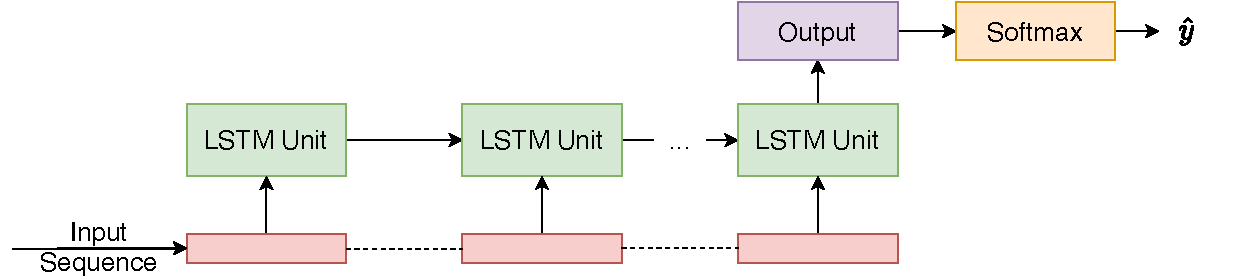
\includegraphics[scale=0.45]{figs/traditional_lstm.pdf}
	\label{fig:LSTM_a}
}\\
	\subfloat[Fingerprint LSTM For Classification]{
	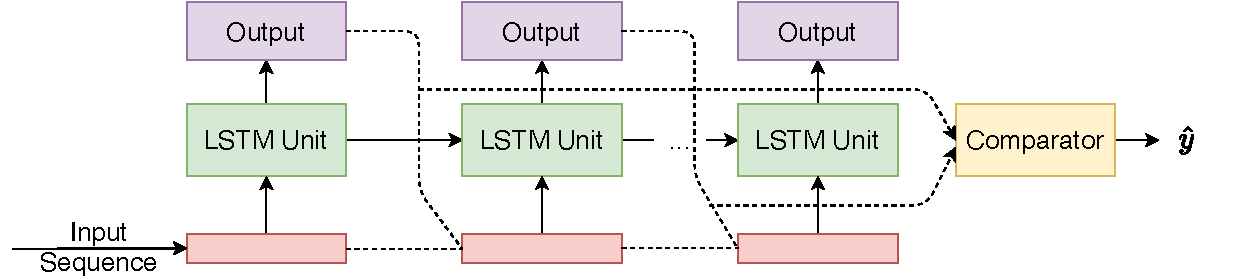
\includegraphics[scale=0.45]{figs/fingerprint_lstm.pdf}
	\label{fig:LSTM_b}
}
	\caption{Comparison between traditional LSTM and fingerprint LSTM.}
	\label{fig:LSTM}
\end{figure}
The LSTM~\cite{hochreiter1997long} is one of the most popular recurrent neural networks (RNNs)~\cite{mandic2001recurrent} to model sequential data. 
LSTM can infer the current state based on the previous state and the current input. 
Therefore, LSTM can remember past information, which is naturally suitable for sequence modeling. 
The main weak point of the vanilla version of RNN is the vanishing/exploding gradient problem which means cannot retain long-term information~\cite{bengio1994learning}. 
By adding gate units with different functions, the LSTM solves the problem. 
It can control the information transformation between the hidden states and track the states of the input sequences without using separate memory cells. 

Traditionally, as shown in Fig.~\ref{fig:LSTM_a},  when LSTM is used for classification tasks, the input sequence is first fed into the LSTM unit. 
Secondly, the output of the last time step of the LSTM unit is given to the fully connected layer.
The classification results can be get after the calculation of the softmax layer. 
However, in this paper, we use our proposed fingerprint LSTM instead of traditional LSTM. 
As shown in Fig~\ref{fig:LSTM_b}, the fingerprint LSTM tries to capture the fingerprints of different types. 
It calculates and compares the loss between the output of the current state and the input of the next time step. 
In the classification stage, the prediction results are determined by the fingerprint LSTM with the minimum loss.
There are two main benefits of fingerprint LSTM. 
First, the traditional LSTM only uses the output of the last time step for the calculation of the fully connected layer. 
Therefore, the traditional LSTM model tends to learn the features of the subsequent input. 
It can be easily affected by noise in the later-arrived packets. 
In the contrast, the learning process of the fingerprint LSTM makes the output of each time step (except the last time step) as close as possible to the input of the next time step. 
This process makes full use of all packets in a session and thus has local robustness. 
Second, a fingerprint LSTM module only characterizes the packet sequence of a specific traffic type. 
The modeling process will not be influenced by other traffic types. 
In the contrast, traditional LSTM may have a bias towards traffic types with a large number of samples.
\section{Proposed Traffic Classification Method}
\label{sec:Proposed_Traffic_Classification_Method}
\begin{figure*}[htbp]
	\centering
	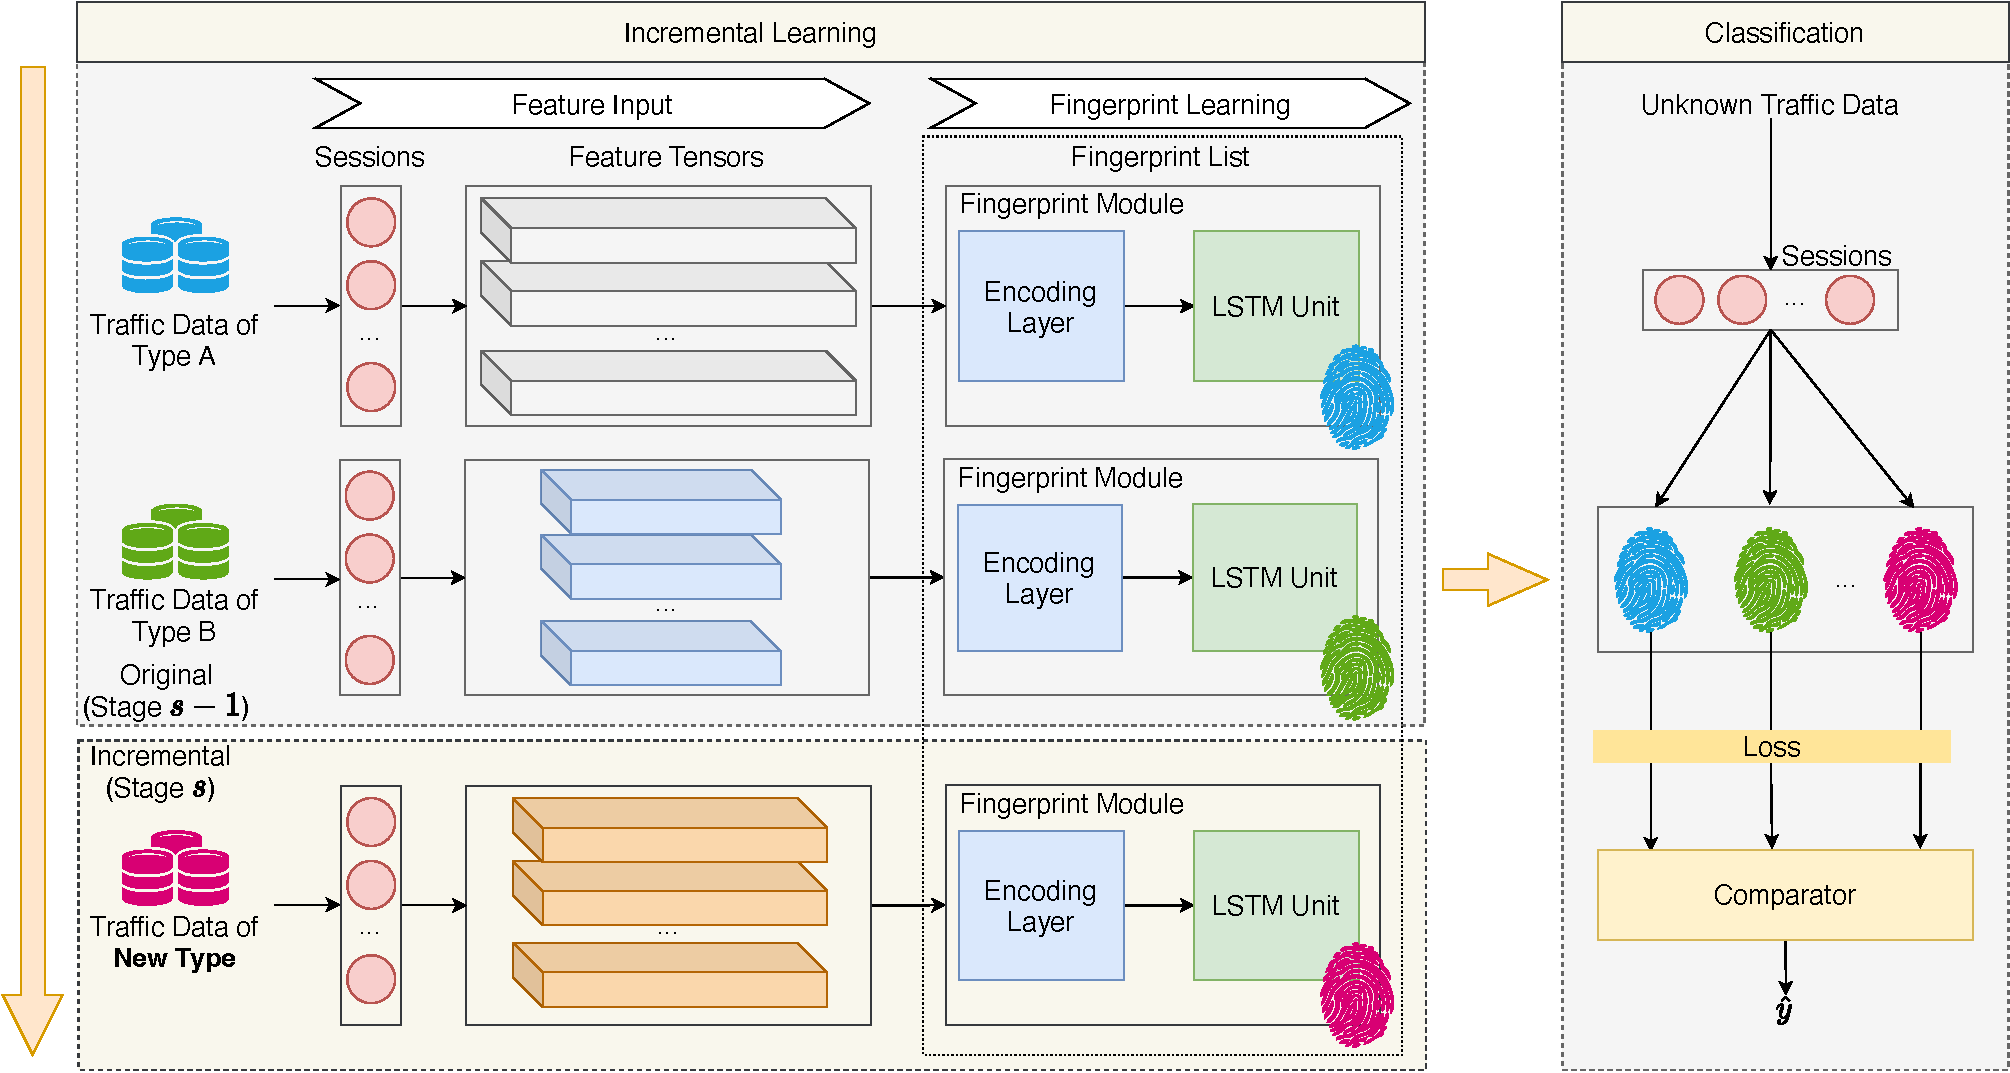
\includegraphics[scale=0.45]{figs/overview_of_model.pdf}
	\caption{Overview of \sys.}
	\label{fig:overview_of_model}
\end{figure*}

\subsection{Overview}
In Section~\ref{sec:Introduction} and Section~\ref{sec:Preliminaries}, we have discussed the limitations of current encrypted traffic classification methods, which motivate us to carry out further studies.
Here we briefly summarize the limitations and motivations as the following two points. 

\first \textit{Current methods for encrypted traffic classification are not suitable for incremental learning.} 
These methods assume the training data for all categories is available at the time of initial training. 
However, it will always emerge new attacks in real-world situations. 
This motivates us to design an incremental model.

\second \textit{Current methods for encrypted traffic classification are not interpretable.} 
The inference process of these methods is under a black-box setting and lacks interpretability. 
However, we need to understand how the model comes to specific conclusions and 
what the model learns.

Based on the above limitations and motivations, we propose the \sys. 
The two main design principles are as follows:

\first \textit{\sys learns the fingerprints of traffic and is interpretable.}
The training process of \sys does not directly implement a traditional classification task. 
Instead, each LSTM unit learns the \emph{fingerprint} (behavioral characteristics) of the input samples. 
In other words, at each time step, the current output of each LSTM unit is as close as possible to the next input of the sequence. 
This learning process is different from the typical classification task which calculates cross-entropy loss at the last time step as described in Section~\ref{sec:Preliminaries}.
We term this training process \emph{fingerprint learning}. 
By such replacement, our \sys has local robustness and is adaptive to imbalanced data.
Moreover, we can rank time-series features, identify import features in prediction and calculate the inter-class distance between different traffic types based on the learning process. 
These capabilities enhance the interpretability of \sys and will be demonstrated in Section~\ref{sec:Model_Interpretability}. 

\second \textit{\sys is an incremental model.} 
It contains multiple independent fingerprint modules. 
Each module maintains a set of parameters and corresponds to the \emph{fingerprint} of a specific traffic type. 
Therefore, we only need to train a set of additional parameters for the newly introduced traffic type. 
Such a design indicates that \sys could be deployed as an incremental model. 

The overview of \sys is depicted in Fig.~\ref{fig:overview_of_model}. 
The whole process of \sys includes incremental learning and classification. 
Further, the workflow of incremental learning can be divided into feature input and incremental fingerprint learning. 
We will discuss each part in detail below.

\subsection{Feature Input}
The first part is feature input. 
In this process, we extract feature tensors from raw traffic data.
We first split the raw traffic data of each traffic type into sessions and then perform feature extraction on each packet in sessions.

For formalization, suppose we have raw traffic data $D$ and we split it into $N$ sessions.
Each session is a sample and is composed of bi-directional packets with the same IP, port, and transport layer protocol.
The feature tensors are extracted from the first $T$ packets in each session and are composed of the packet feature vectors. 
Each packet feature vector consists of packet length, direction, the interval of arrival time, and values of fields in the packet header, \eg TTL (Time To Live), TCP flags, and TCP window size. 
Therefore, the feature tensor of the $p$-th sample can be denoted as $\mathbf{x^{(p)}} = [\mathbf{L_1^{(p)}}, \mathbf{L_2^{(p)}}, ..., \mathbf{L_T^{(p)}}]$, where $T$ is the time sequence length of each sample and $\mathbf{L_i^{(p)}} \in \mathbb{R}^d$ is the $d$-dimensional packet feature vector at time step $i$. 

Particularly, the flexibility of our feature input is that we can select different features and different time sequence lengths for each traffic type, \ie $d$ and $T$ can be different for various traffic types.  
In other words, the feature input process is not dependent on the fixed number of traffic types. 
When a new traffic type is added, we can select the appropriate features and time sequence length for this newly added traffic type without affecting those of existing traffic types.
This property of the feature input process creates the conditions for incremental fingerprint learning.

\subsection{Incremental Fingerprint Learning}
The second part is incremental fingerprint learning. 
In this process, we learn the fingerprints of different traffic types in an incremental manner.

Different from the model training process of typical classification tasks with LSTM, \sys aims to train a model which can learn \emph{fingerprints} (behavioral characteristics) of each traffic type. 
We call this process \emph{fingerprint learning}. 
As described in previous sections, we use fingerprint LSTM instead of traditional LSTM to model the packet sequence in sessions of a traffic type, which has local robustness and is suitable for an imbalanced dataset.

In addition, we add an encoding layer before fingerprint LSTM to constitute a fingerprint module.
The encoding layer takes the original feature tensors as input and generates the latent representations.
It simply uses a linear layer with the $\mathit{tanh}$ activation function.
There are two benefits of adding an encoding layer.
\first Some fields in the packet headers are categorical features, \eg TCP Flags (SYN, ACK, etc). The encoding layer can transform these features into numerical features, which are more convenient for computation.
\second There may be redundant information in the original features. 
The encoding layer can reduce the redundant information, which helps the model learn the fingerprints of network traffic better. 

Moreover, the \sys maintains a fingerprint list. 
As depicted in Fig.~\ref{fig:overview_of_model}, there are multiple fingerprint modules in the fingerprint list. 
Each fingerprint module maintains an \emph{independent} set of parameters that corresponds to a traffic type.
This means that \sys is designed in an incremental learning manner. 
In other words, the only thing that needs to be done for having the ability to recognize a new traffic type is to introduce an additional fingerprint module to the fingerprint list and to train this module with the new traffic data.
This provides \sys the capability to classify new traffic types, without retraining existing fingerprint modules.

The entire algorithm of incremental fingerprint learning is exhibited in Algorithm~\ref{alg:incremental_fingerprint_learning}.
\begin{algorithm}[H]
\caption{Incremental Fingerprint Learning.}
\label{alg:incremental_fingerprint_learning}
\renewcommand{\algorithmicrequire}{\textbf{Input:}}
\renewcommand{\algorithmicensure}{\textbf{Output:}}
\begin{algorithmic}[1]
\REQUIRE $X^s, \psi^{s-1}$
\STATE Create a new fingerprint module $[\rho^s, \Omega^s]$
\STATE Initialize the parameters of $[\rho^s$, $\Omega^s]$ randomly
\FOR{$\mathbf{x^{(p)}} \in D^s$} 
	\STATE $\mathbf{e^{(p)}} \gets \rho^s(\mathbf{x^{(p)}}) $
	\STATE $\mathbf{a^{(p)}} \gets \Omega^s(\mathbf{e^{(p)}})$
	\STATE $\mathcal{L}(\mathbf{x^{(p)}}) \gets \frac{1}{T-1} \sum_{t=1}^{T-1}\vert\vert \mathbf{a_t^{(p)}} - \mathbf{L_{t+1}^{(p)}} \vert\vert $
	\STATE Calculate the gradient of parameters of $[\rho^s, \Omega^s]$
	\STATE Update the parameters of $[\rho^s, \Omega^s]$
\ENDFOR
\STATE $\psi^s \gets $ append $[\rho^s, \Omega^s]$ to the fingerprint list of $\psi^{s-1}$
\ENSURE $\psi^{s}$
\end{algorithmic}
\end{algorithm}

In an incremental learning scenario, we introduce a new traffic type using training samples $X^s$.
After the incremental fingerprint learning, the previous stage model $\psi^{s-1}$ becomes $\psi^s$, which has the ability to classify the new traffic type.
The first step of incremental fingerprint learning is to create a new fingerprint module, which consists of an encoding layer $\rho^s$ and a fingerprint LSTM $\Omega^s$ (line 1).
Then we randomly initialize the parameters of each component of the fingerprint module (line 2). 
In each iteration, we sequentially feed the training samples into the encoding layer and the fingerprint LSTM (lines 4-5). 
The learning process aims to make the output $\mathbf{a_t^{(p)}}$ as close as possible to the next input $\mathbf{L_{t+1}^{(p)}}$ at $t$-th time step,  where $1 \le t \le T-1 $ (line 6). 
Therefore, the loss function of the $p$-th sample can be set as follow: 
\begin{equation}\label{eq:lossfunction}
    \mathcal{L}(\mathbf{x^{(p)}}) = \frac{1}{T-1} \sum_{t=1}^{T-1}\vert\vert \mathbf{a_t^{(p)}} - \mathbf{L_{t+1}^{(p)}} \vert\vert
\end{equation}
After the calculation of loss, we can obtain the gradient of the parameters of the fingerprint module with backpropagation (line 7). 
Then we update the parameters of the fingerprint module (line 8).
We can get the new model $\psi^s$ after iterations over all training samples (line 10).

\subsection{Traffic Classification}
The third part is the traffic classification. 
When the unknown traffic data arrives,  we first process the data with feature input, which converts the raw traffic data into feature tensors. 
Then we feed feature tensors to each fingerprint module in the fingerprint list that is trained in the incremental fingerprint learning part.
Each fingerprint module calculates the loss defined in Eq.~(\ref{eq:lossfunction}).
Since each fingerprint module has learned the \emph{fingerprint} of a specific traffic type, it will output a small loss for traffic with exactly the same type while giving a relatively large loss for the sample of other traffic types. 
Consequently, the unknown traffic is classified as the corresponding type of the fingerprint module with the minimum loss.
This process is represented as a \emph{comparator} in Fig.~\ref{fig:overview_of_model}.
To formulate this process, suppose that $\mathcal{L}_i(\mathbf{x^{(p)}})$ represents the output loss of $p$-th unknown traffic sample calculated by $i$-th fingerprint module in the fingerprint list. We can classify the sample as $\hat{y_p}$ by determining the specific $i$ which makes $\mathcal{L}_i(\mathbf{x^{(p)}})$ minimum,
\begin{equation}\label{eq:argminlabel}
\hat{y_p} = \mathop{\arg\min}\limits_{i}  \mathcal{L}_i(\mathbf{x^{(p)}})
\end{equation}

\section{Model Interpretability}
\label{sec:Model_Interpretability}
In the previous section, we have described the design of \sys. In this section, we elaborate on the model interpretability of \sys from the aspects of feature attribution and inter-class distance between traffic types. 

\subsection{Sequence Feature Attribution}
\label{sec:Sequence_Feature_Ranking}
Feature attribution is an important part of model interpretability, which can be divided into global-level attribution and local-level attribution.
The result of the global level attribution is usually the feature ranking of a specific type, while the local level attribution mainly gives the importance of each feature in the prediction of a single sample.

However, existing feature attribution methods are mainly applicable to tabular data and are not designed for network traffic data, which is time series.
If we want these existing feature attribution algorithms to handle the network traffic data, we need to convert the time-series data to tabular data.
A common way to accomplish the above transformation is to reshape the time sequence data.
For example, assume the time sequence data $a$ has a total of $T$ time steps, and each time step is a $d$-dimensional feature vector. We can use \texttt{b = a.reshape(1, $T\times d$)} to reshape the time sequence data $a$ to tabular data $b$ with \textit{NumPy}~\cite{harris2020array}. 
However, this way has two shortages. 
\first This transformation considers features at each time step individually and ignores the relationship between the time sequence data.
\second Current feature ranking methods need a long computation time and have a scalability problem to handle the high-dimensional reshaped data~\cite{zou2016novel}. 

To address the feature attribution of network traffic data, we propose an effective sequence feature attribution method based on \sys.
The interpretability of \sys focuses on the influence of features on fingerprints in terms of time sequence. 
Therefore, \sys provides a new perspective that illustrates the attribution of sequence features.

\begin{figure}[htbp]
	\centering
	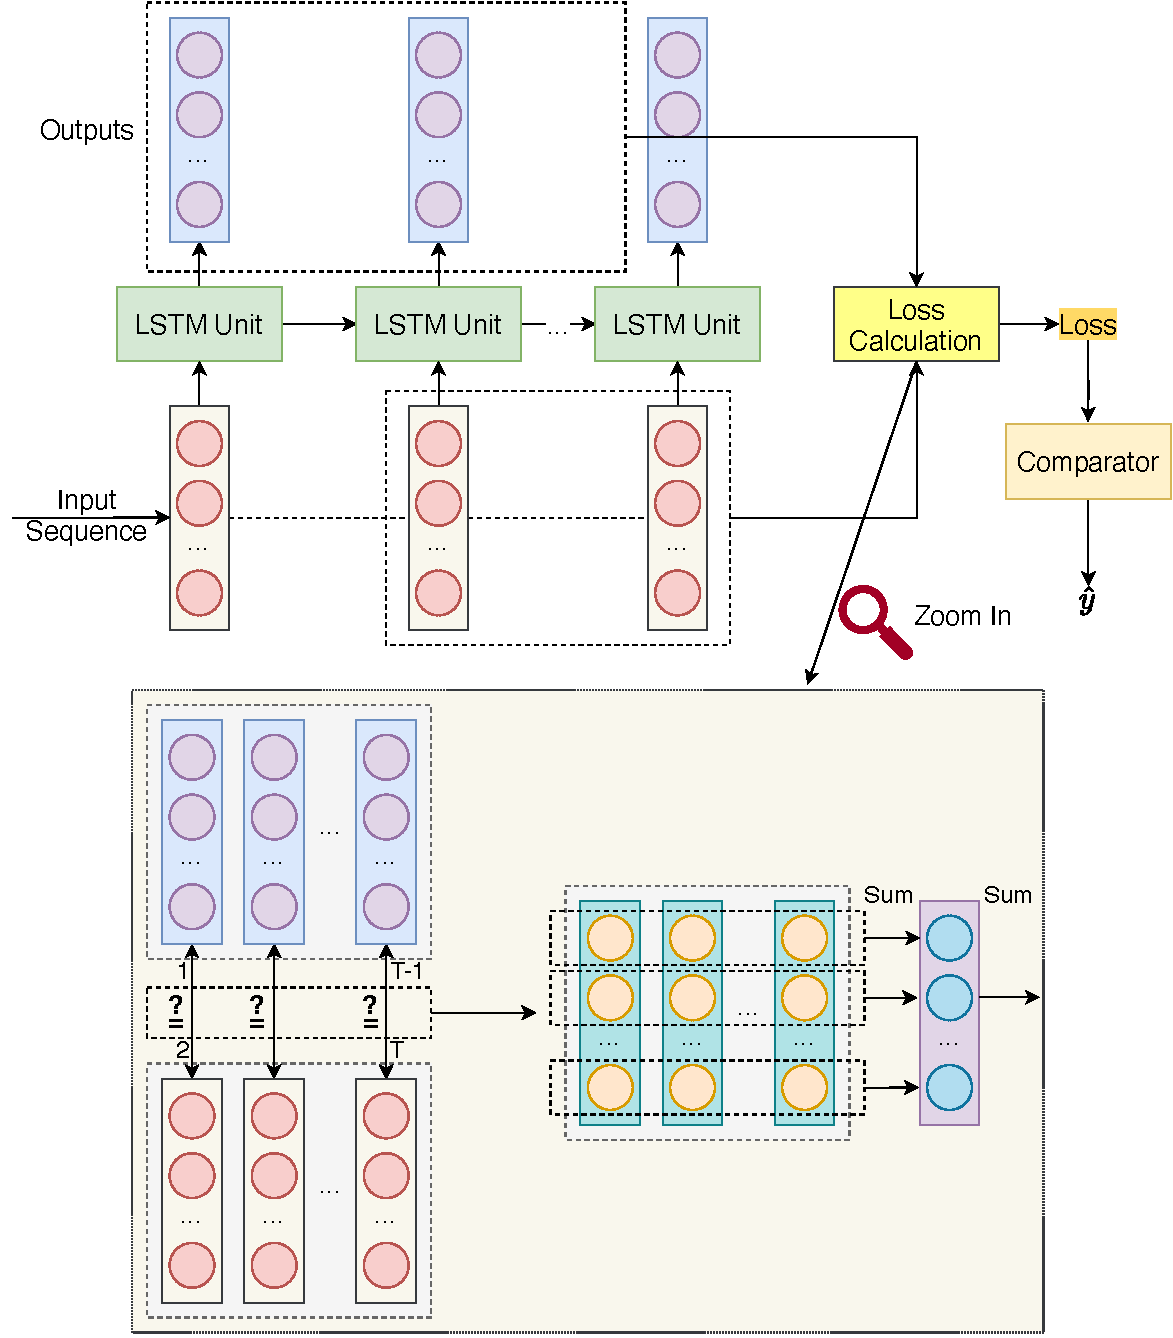
\includegraphics[scale=0.45]{figs/interpretability.pdf}
	\caption{Internal computational process of \sys.}
	\label{fig:interpretability}
\end{figure}

Our feature attribution method stems from the decomposition of the internal computational process of \sys.
Fig.~\ref{fig:interpretability} illustrates the internal computational process of \sys when feeding traffic sequence data.
As mentioned in Section~\ref{sec:Proposed_Traffic_Classification_Method}, each fingerprint module is trained to learn the \emph{fingerprint} (behavioral characteristics) of a specific traffic type and the classification result of the unknown traffic is decided by the fingerprint module with the minimum loss. 
At each time step, the fingerprint module outputs the prediction of the next time step based on the previous input. 
The loss is computed according to Eq.~(\ref{eq:lossfunction}).
Actually, Eq.~(\ref{eq:lossfunction}) is equivalent to first calculating the L2 distance between the output vector and the next input vector at each time step and then summing the distance of each dimension.
Specifically, each dimension of $\mathbf{a_t^{(p)}} - \mathbf{L_{t+1}^{(p)}}$ jointly contributes to the overall loss in Eq.~\eqref{eq:lossfunction}.
Therefore, for a specific traffic type, compared the loss at a certain dimension of the corresponding fingerprint module with losses of other fingerprint modules at the same dimension, if the loss at this dimension is smaller and thus has a larger loss difference, we can say this dimension contributes more to the final prediction and thus ranks higher.
This is the basic idea of our feature attribution method. 
Practically, we feed data of a specific type to all the fingerprint modules in the fingerprint list of \sys. 
We calculate the sum of loss difference in each dimension among fingerprint modules and use it to represent the feature importance.

For formalization, we first define the single-dimensional loss of a sample as
\begin{equation}\label{eq:single-dimensional_loss_sample}
    \mathcal{SL}(\mathbf{x^{(p)}},  \psi_J,  K) = \frac{1}{T-1} \sum_{t=1}^{T-1}\vert \mathbf{a_{J, t}^{(p)}}[K] - \mathbf{L_{t+1}^{(p)}}[K] \vert
\end{equation}
where $\mathcal{SL}(\mathbf{x^{(p)}},  \psi_J,  K)$ represents the $K$-th dimensional loss when feeding sample $\mathbf{x^{(p)}}$ into the $J$-th fingerprint module in the fingerprint list.  
Subsequently, we can calculate the loss difference between fingerprint modules in the $K$-th dimension of a sample $\mathbf{x^{(p)}}$ (abbreviated as feature loss) as follows,
\begin{equation}\label{eq:feature_loss_sample}
\begin{split}
    \mathcal{FL}(\mathbf{x^{(p)}}, K) &= \frac{1}{M}\sum_{J=0}^{M-1} ReLU(\mathcal{SL}(\mathbf{x^{(p)}},  \psi_J,  K) \\
&- \mathcal{SL}(\mathbf{x^{(p)}},  \psi_I,  K))
\end{split}
\end{equation}

The $I$-th fingerprint module only learns the \emph{fingerprint} of traffic type $I$, which is the corresponding type of sample $\mathbf{x^{(p)}}$. 
Consequently, if $I \neq J$, the overall loss $\mathcal{L}_I(\mathbf{x^{(p)}})$ is supposed to be less than $\mathcal{L}_J(\mathbf{x^{(p)}})$, and $K$-th dimension loss $\mathcal{SL}(\mathbf{x^{(p)}},  \psi_I,  K) $ should be less than $\mathcal{SL}(\mathbf{x^{(p)}},  \psi_J,  K) $ correspondingly. 
Therefore, $\mathcal{FL}(\mathbf{x^{(p)}}, K)$ is usually a positive value.  
We use ReLU~\cite{nair2010rectified} to get the non-negative part. 
A larger value indicates that the feature at this dimension contributes more to the difference in the overall loss that the traffic classification relies on. 
Thus we consider the value $\mathcal{FL}(X^I, K)$ as the significance of the feature at the $K$-th dimension of a sample $\mathbf{x^{(p)}}$.

Eq.~\eqref{eq:single-dimensional_loss_sample} and Eq.~\eqref{eq:feature_loss_sample} define the feature importance of a single sample, which offer local interpretability.
For the global interpretability of \sys, we can sum the feature importance of all the samples belonging to traffic type $I$,
\begin{equation}\label{eq:single-dimensional_loss}
\mathcal{SL}(X^I,  \psi_J,  K) = \sum_{\hat{y^{(p)}}=I}\mathcal{SL}(\mathbf{x^{(p)}},  \psi_J,  K) 
\end{equation}
\begin{equation}\label{eq:feature_loss}
\mathcal{FL}(X^I, K) = \sum_{\hat{y^{(p)}}=I} \mathcal{FL}(\mathbf{x^{(p)}}, K)
\end{equation}

\begin{figure}[htbp]
	\centering
	\subfloat[Feature ranking for each traffic type.]{
		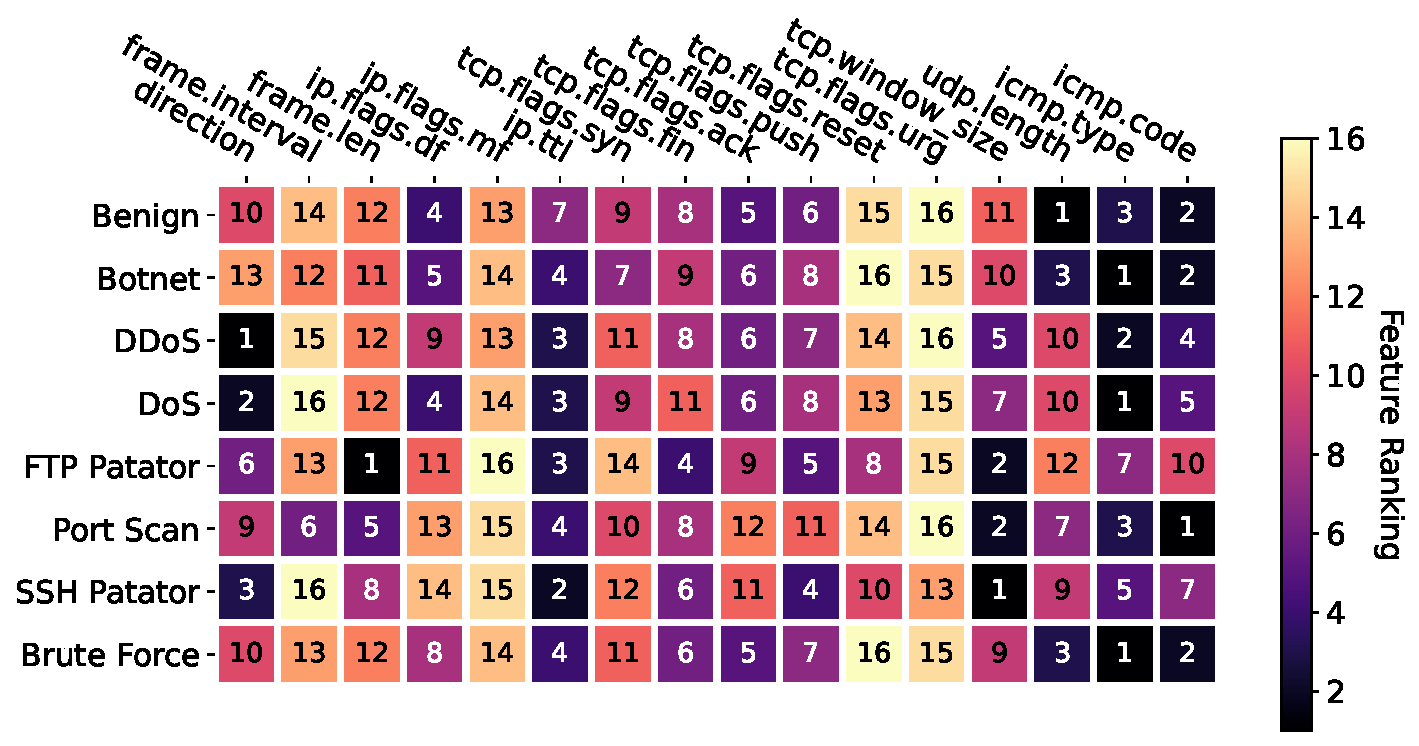
\includegraphics[width=0.95\linewidth]{figs/fingerprint_ids_fingerprint_rank.pdf}
		\label{fig:global_interpret}
	}\\
	\subfloat[Feature importance for classification of traffic samples.]{
		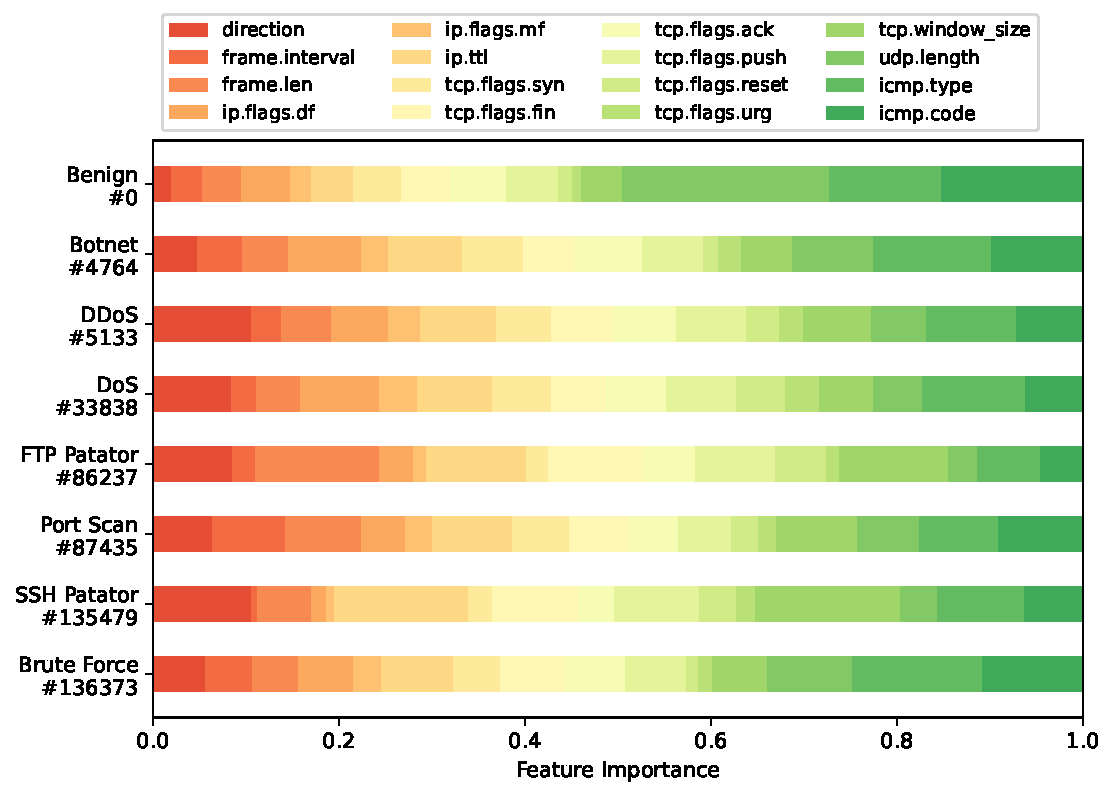
\includegraphics[width=0.95\linewidth]{figs/fingerprint_local_importance.pdf}
		\label{fig:local_interpret}
	}
	\caption{An example of feature attribution results.}
	\label{fig:fea_interpretability}
\end{figure}

Fig.~\ref{fig:fea_interpretability} shows an example of the feature attribution results. 
Fig.~\ref{fig:global_interpret} depicts the feature ranking results for each traffic type.
Each row represents a specific traffic type.
Each column stands for a specific feature.
The numbers inside the square represent the feature ranking (smaller is higher).
These results are interpretable from the perspective of attack principles.
For example, from Fig.~\ref{fig:global_interpret}, we can see that the \emph{direction} is the significant feature for DDoS and DoS.
This is because the communication pattern of these two traffic types is mainly the attacker (the client) sending a flood of packets to the server.
Fig.~\ref{fig:local_interpret} shows the feature importance of samples, illustrating which features contribute more to the classification results.
The numbers on the y-axis are indexes of the selected sample on the dataset. 
It facilitates us to understand how the model comes to the final prediction results.
Take the FTP Patator \#86237 as an example,  we can see that the \emph{frame.len} plays an important role in the classification.
This is mainly because the purpose of the FTP Patator is to keep trying to decipher the password of the FTP server.
Meanwhile, the packet length of the authentication process in FTP is always a fixed value. 

\subsection{Inter-Class Distance between Traffic Types}
\label{sec:inter_class_distance}
According to our design of fingerprint learning, the fingerprint module will output a larger loss if we feed traffic data whose type is not the corresponding type of the fingerprint module.
In other words, the loss is the distance between the input traffic and the expected traffic of the fingerprint module.
In the previous section, we have defined the single-dimensional loss $\mathcal{SL}(X^I,  \psi_J,  K)$ in Eq.(\ref{eq:single-dimensional_loss}), which is the $K$-th dimension of the output loss when feeding traffic data of type $I$ into the $J$-th fingerprint module. 
Based on this, we define the inter-class distance from traffic type $I$ to traffic type $J$ at dimension $K$ as
\begin{equation}\label{equ:traffic_distance}
    \mathcal{DI}(I, J, K) = ReLU(\mathcal{SL}(X^I,  \psi_J,  K) - \mathcal{SL}(X^I,  \psi_I,  K))
\end{equation}
The inter-class distance actually reflects the similarity between traffic types. 
Considering that the distance is always the non-negative value, we use ReLU to extract the non-negative part.
If we take each traffic type as a point and express the distance between the traffic types as an edge between the points, we can draw the distance map on a two-dimensional plane.
Note that in general $\mathcal{DI}(I, J, K) \neq \mathcal{DI}(J, I, K)$ and thus the distance map should be a directed graph. 

\begin{figure}[htbp]
	\centering
	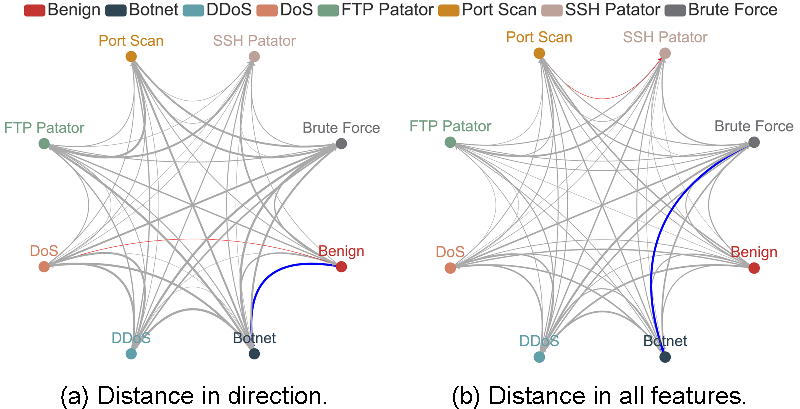
\includegraphics[scale=0.6]{figs/inter_class_distance.pdf}
	\caption{An example of the inter-class distance between traffic types.}
	\label{fig:traffic_distance}
\end{figure}

Fig.~\ref{fig:traffic_distance} shows an example of the inter-class distance between traffic types. 
We use a larger linewidth to represent a smaller inter-class distance. 
In each subfigure, the red and blue lines indicate the largest and smallest inter-class distances, respectively. 
Due to the page limitation, we only present the inter-class distance in the dimension of direction and in all features.
We find the results are rational.
For example, we can see that Port Scan and Brute Force are close in direction. 
This is mainly because the behavior of these two traffic types is similar, \ie attempting to access information about the server by sending massive packets to the target in a short time.
DoS and DDoS are close to each other in all features due to their similar attack behaviors.
Particularly, Benign and Botnet are the closest in direction because they are both bidirectional communication between the client and servers. 
In contrast, DoS and Benign are the farthest in direction as the DoS traffic is usually from clients to the target server while Benign contains bidirectional flows. 
Moreover, we can observe that Botnet and Brute Force are the closest while Port Scan and SSH Patator are the farthest in all features. 
Inspired by this result, we try to group the traffic types with close distances to a new individual type, which may reduce the struggle of the model to distinguish between similar types and improve the classification performance of the model. 
The details of this experiment can be found in Section~\ref{sec:group}.

\section{Evaluation}
\label{sec:Evaluation}
In this section, we present the experimental settings and the evaluation results of the proposed \sys.

\subsection{Experimental Settings}
\subsubsection{Datasets}
We evaluate the proposed \sys on two public datasets CIC-IDS2017 dataset~\cite{sharafaldin2018toward} and ISCXVPN2016 traffic dataset~\cite{draper2016characterization}, respectively. 
The first dataset contains the hybrid of encrypted and unencrypted network traffic across five days, which can be divided into 8 classes, Benign, FTP Patator, SSH Patator, DoS, Web Brute Force, Botnet, Port Scan, and DDoS respectively.
The second dataset contains pure encrypted traffic, which is composed of 14 applications, \eg Facebook, Netflix, Skype, etc.
The applications are encrypted with various security protocols, including HTTPS, SSH, and proprietary protocols.
Both two datasets are imbalanced.
For example, in the CIC-IDS2017 dataset, Port Scan accounts for 35.07\%, while Botnet only accounts for 0.27\%.
In the ISCXVPN2016 traffic dataset, Email accounts for 16.89\%, while SFTP only accounts for 0.65\%. 

\subsubsection{Baselines}
We compare \sys against various baseline works for encrypted traffic classification, including KNN~\cite{mcgaughey2018systematic}, RF~\cite{zhai2018random}, MLP~\cite{aceto2018mobile}, LSTM~\cite{vu2018time}, and FS-Net~\cite{liu2019fs}. 

We compare our global feature ranking method against the mutual information feature ranking~\cite{kraskov2004estimating}, RFE feature ranking~\cite{guyon2002gene}, and random forest feature ranking~\cite{louppe2014understanding}.  
Since these methods cannot be performed on time-series features directly, we first reshape the time-series data into tabular data as mentioned in Section~\ref{sec:Sequence_Feature_Ranking}.
Then we calculate the feature importance on the reshaped data with these methods respectively.  
Finally, we \emph{restore} the results of feature importance to the corresponding time-series features to obtain the feature ranking of the original features.
The process \emph{restore} is to accumulate the feature importance of corresponding features on the reshaped data, for each feature of the original time-series data.

In terms of local interpretability, we compare the performance of our proposed method against well-known methods, including LIME~\cite{lime}, SHAP~\cite{shap}, and Feature Permutation~\cite{altmann2010permutation}.

\subsubsection{Implementation Details}
The time sequence length of each LSTM unit is set as 32.  
We set the dimension of the encoding layer as 8.
The dimension of hidden states of each fingerprint LSTM is set as 16.
The Adam optimizer~\cite{kingma2014adam} with a learning rate of 0.001 is used.  
Our proposed method \sys is implemented with \emph{PyTorch}. %~\cite{paszke2019pytorch}.
We use \emph{scikit-learn}~\cite{scikit-learn} to implement other compared methods.
The compared local interpretability methods are the implementation from \emph{Captum}~\cite{kokhlikyan2020captum}.
All experiments in this paper are conducted using a 12-core PC with an NVIDIA GeForce GTX 1070 GPU, 128GB of RAM, and Ubuntu 16.04 LTS.

\subsubsection{Evaluation Metrics}
We evaluate the classification performance of \sys with other baselines in terms of Accuracy (AC), Precision (PR), Recall (RC), and F1-Score (F1)~\cite{zheng2020learning}.
Macro Average~\cite{liu2017efficient} is used to avoid biased results due to imbalance between multiple categories of data by calculating the mean value of AC, PR, RC, and F1 of each category.

The performance of local interpretability will be evaluated in terms of stability, robustness, and effectiveness~\cite{fan2020can}.

\subsection{Evaluation of Classification}
In this section, we evaluate \sys and baseline classification methods with the 5-fold cross-validation.

\subsubsection{Effectiveness of the Fingerprint Learning}
\begin{figure*}[htbp]
	\centering
	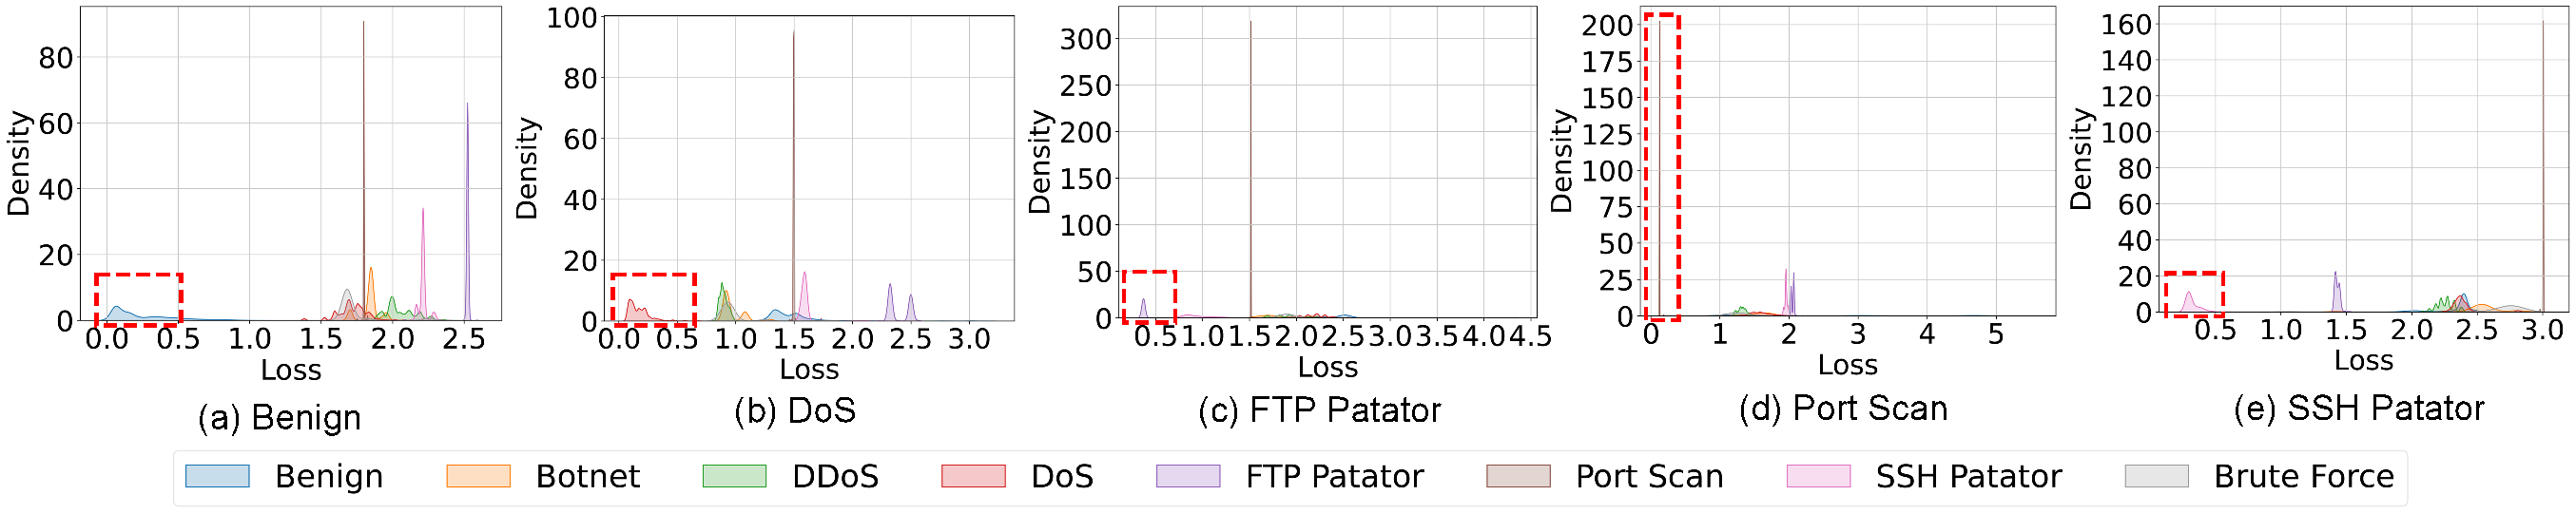
\includegraphics[scale=0.4]{figs/loss_kde.pdf}
	\caption{KDE of losses output by fingerprint modules when feeding different types of traffic data on CIC-IDS2017.}
	\label{fig:loss_kde}
\end{figure*}
In order to show the effectiveness of fingerprint learning, we plot the distribution of losses output by each fingerprint module when feeding traffic data of different types.
Each subfigure in Fig.~\ref{fig:loss_kde} shows the kernel density estimation (KDE)~\cite{silverman2018density} of the distribution of losses (due to page limitation we do not show all results).
The losses of samples whose types are exactly the corresponding type of the fingerprint module (red rectangle part) are significantly lower than that of other types (x-axis). 
It demonstrates that each fingerprint module in the fingerprint list of \sys can learn the \emph{fingerprint} of the corresponding traffic type well. 
In other words, the core idea of \sys described in Section~\ref{sec:Proposed_Traffic_Classification_Method} is effective. 

Table~\ref{tab:classification_ids} and Table~\ref{tab:classification_vpn} show the classification results. 
It is clear that \sys achieves significant classification performance and outperforms all other methods in both traffic datasets.
The KNN, RF, and MLP are designed to learn from the tabular data. 
They cannot model the context information in the sequence data and thus perform worse than \sys.
The \sys has a better classification performance than LSTM and FS-Net, especially in F1-Score.
It is mainly because both datasets are imbalanced.
The \sys leverages the advantage of fingerprint learning, \ie each fingerprint module is only responsible for identifying one traffic type. 
Thus it will not be confused by different traffic fingerprints and is suitable for imbalanced data. 

\begin{table}[htbp]
\centering
\caption{Comparison Results of Different Classification Methods on CIC-IDS2017 dataset}
\label{tab:classification_ids}
\begin{tabular}{|c|c|c|c|c|} 
\hline
Method       & AC     & PR     & RC     & F1     \\
\hline
\textbf{I2RNN}        & \textbf{0.9897} & \textbf{0.9864} & \textbf{0.9859} & \textbf{0.9861} \\
\textbf{I2RNN w/o EL} & 0.9769 & 0.9752 & 0.9729 & 0.9766 \\
\hline
KNN~\cite{mcgaughey2018systematic}          & 0.9579 & 0.8886 & 0.8891 & 0.8886 \\
RF~\cite{zhai2018random}           & 0.9698 & 0.9692 & 0.9621 & 0.9629 \\
MLP~\cite{aceto2018mobile}          & 0.9699 & 0.9699 & 0.9693 & 0.9630 \\
LSTM~\cite{vu2018time}         & 0.9649 & 0.7961 & 0.8560 & 0.8124 \\
FS-Net~\cite{liu2019fs}       & 0.9526 & 0.4721 & 0.4439 & 0.4218 \\
\hline
\end{tabular}
\end{table}

\begin{table}[htbp]
\centering
\caption{Comparison Results of Different Classification Methods on ISCXVPN2016 dataset}
\label{tab:classification_vpn}
\begin{tabular}{|c|c|c|c|c|}
\hline
Method       & AC     & PR     & RC     & F1     \\
\hline
\textbf{I2RNN}        & \textbf{0.9393} & \textbf{0.9068} & \textbf{0.9178} & \textbf{0.9013} \\
\textbf{I2RNN w/o EL} & 0.8922 & 0.8683 & 0.8693 & 0.8490 \\
\hline
KNN~\cite{mcgaughey2018systematic}          & 0.8799 & 0.7692 & 0.7094 & 0.6924 \\
RF~\cite{zhai2018random}           & 0.8712 & 0.8742 & 0.8647 & 0.8634 \\
MLP~\cite{aceto2018mobile}          & 0.8503 & 0.6992 & 0.6745 & 0.5540 \\
LSTM~\cite{vu2018time}         & 0.8813 & 0.5213 & 0.5132 & 0.5006 \\
FS-Net~\cite{liu2019fs}       & 0.5230 & 0.0924 & 0.1122 & 0.0859 \\
\hline
\end{tabular}
\end{table}

\subsubsection{Local Robustness of the Fingerprint Learning}
We compare the local robustness of the fingerprint learning of \sys and traditional classification with LSTM when having noise in packet sequence.
We add a Gaussian noise $\epsilon~N(0, 1)$ with different perturbation ratios $\beta \in [0, 1]$ to the last two packets in the packet sequence of a session.
The experiment results are shown in Fig.~\ref{fig:perturbation}.
When gradually increasing the perturbation ratio from 0.0 to 1.0, we find the accuracy and F1-Score of the fingerprint LSTM change slightly while the performance of the traditional LSTM drops sharply. 
This result indicates our fingerprint LSTM has local robustness and is more stable in face of noises in sessions.
\begin{figure}[htbp]
	\centering
	\subfloat{
		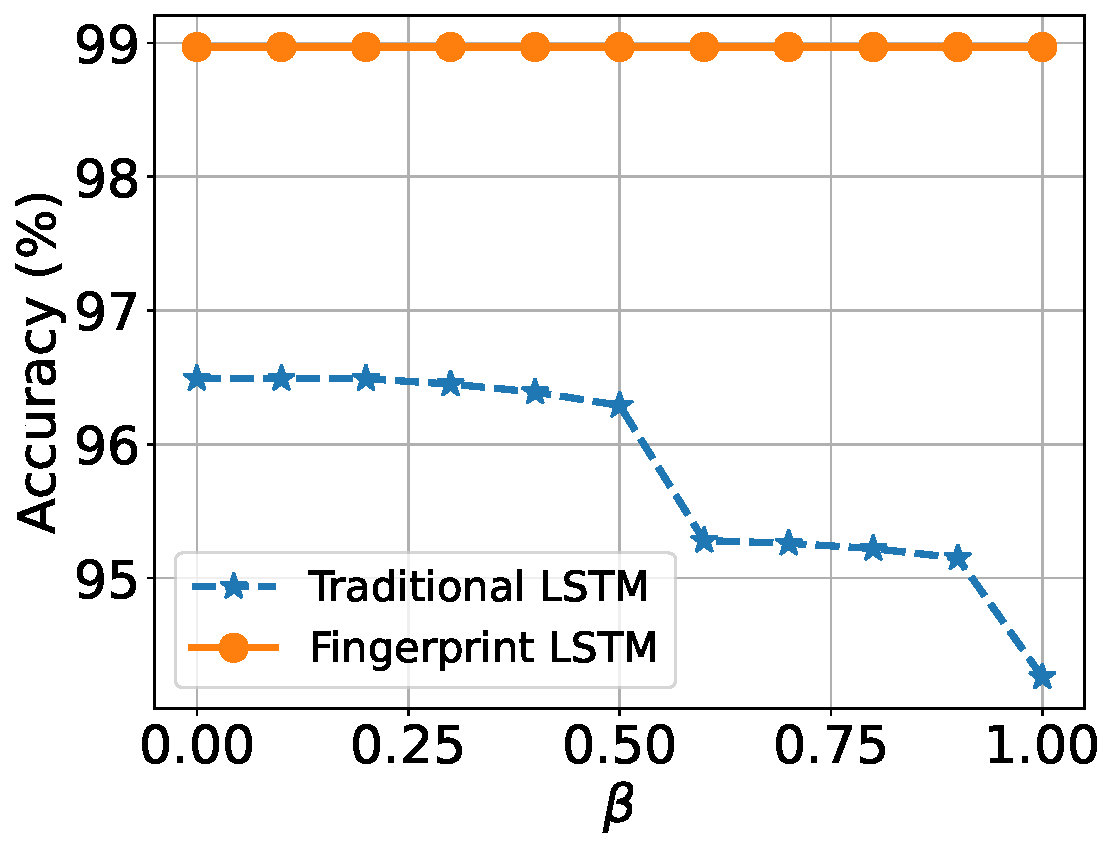
\includegraphics[width=0.47\linewidth]{figs/ids_perturbation_acc.pdf}
	}\hfill
	\subfloat{
		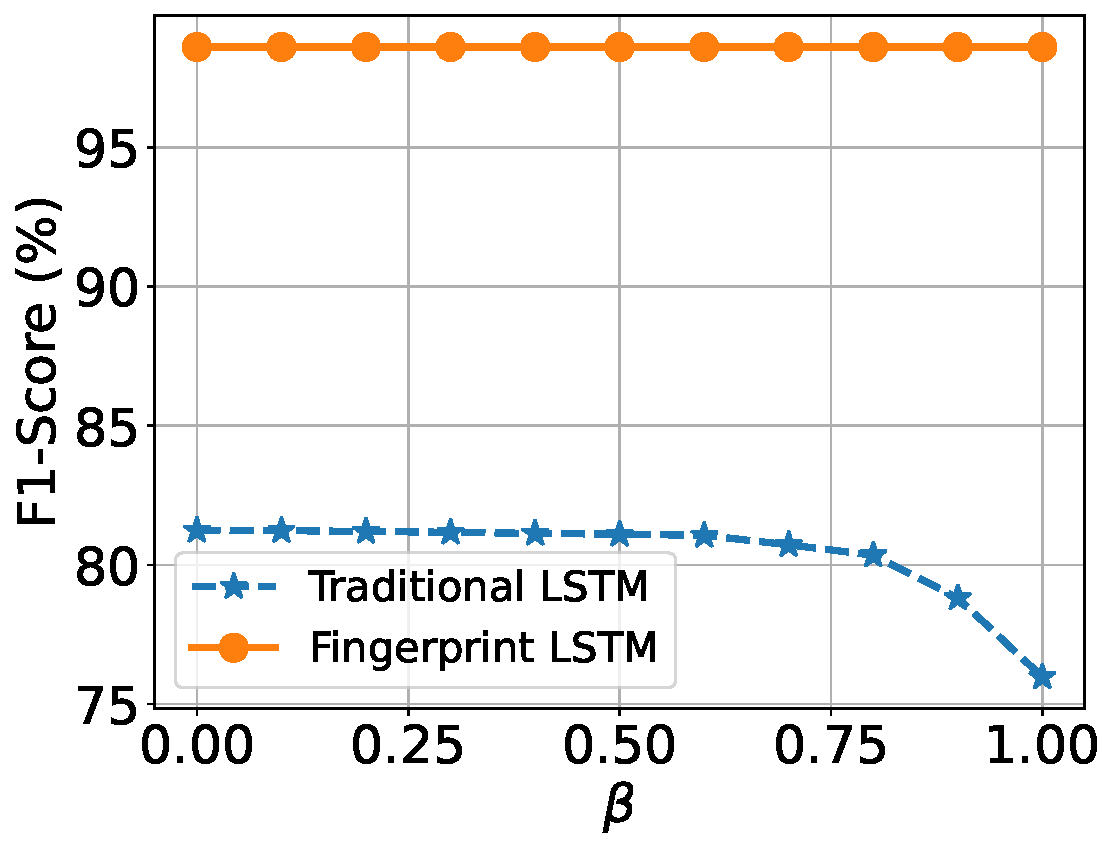
\includegraphics[width=0.47\linewidth]{figs/ids_perturbation_f1.pdf}
	}
	\caption{Comparison results of traditional LSTM and fingerprint LSTM on CIC-IDS2017 with different perturbation ratios $\beta$.}
	\label{fig:perturbation}
\end{figure}

\subsubsection{Ablation Study of the Encoding Layer}
To verify the effectiveness of the encoding layer, we train a variant version of \sys without the encoding layer (EL), which is termed as \sys w/o EL in Table~\ref{tab:classification_ids} and Table~\ref{tab:classification_vpn}.
We can see that the \sys with the encoding layer has a better performance than the variant version of \sys without the encoding layer. 
This result indicates that the encoding layer has effects on categorical feature transformation and redundant information reduction. 

\subsection{Evaluation of Incremental Learning}

\subsubsection{Comparison of Training Time and Preserved Data Size}
\label{sec:inc_time_size}
Fig.~\ref{fig:inc_time_size} presents the comparison of the training time and the size of data needed to be preserved when giving different numbers of incremental data.
Compared to the traditional LSTM, our proposed fingerprint LSTM is more efficient in training time and the size of data needed to be preserved under an incremental learning scenario. 

\begin{figure}[htbp]
	\centering
	\subfloat{
		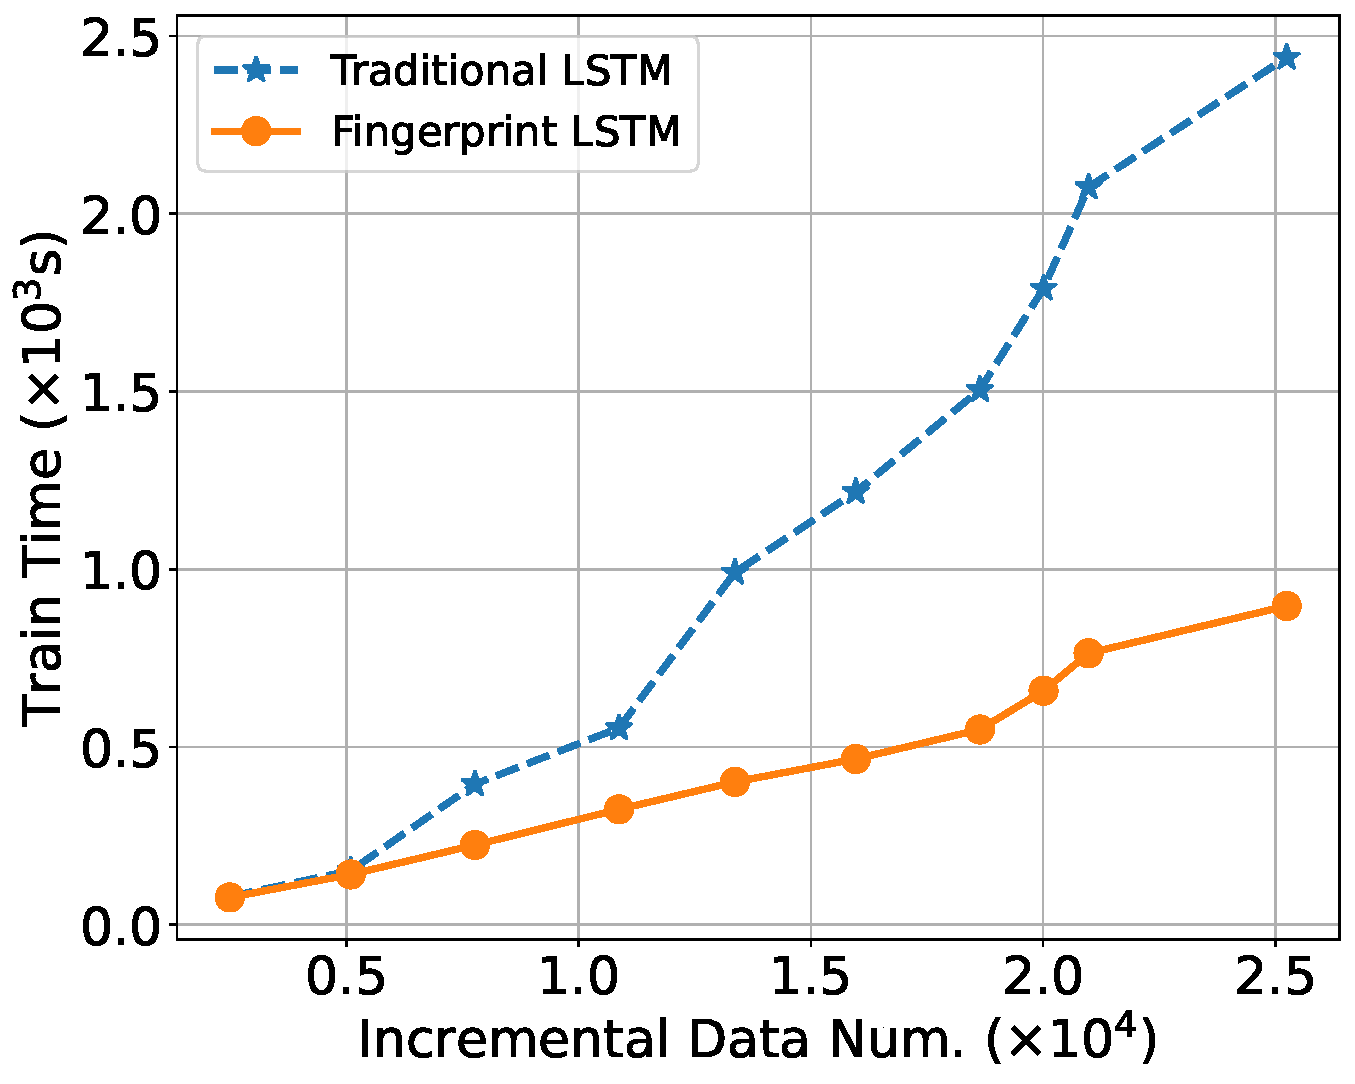
\includegraphics[width=0.47\linewidth]{figs/inc_time_size_cmp_time.pdf}
	}\hfill
	\subfloat{
		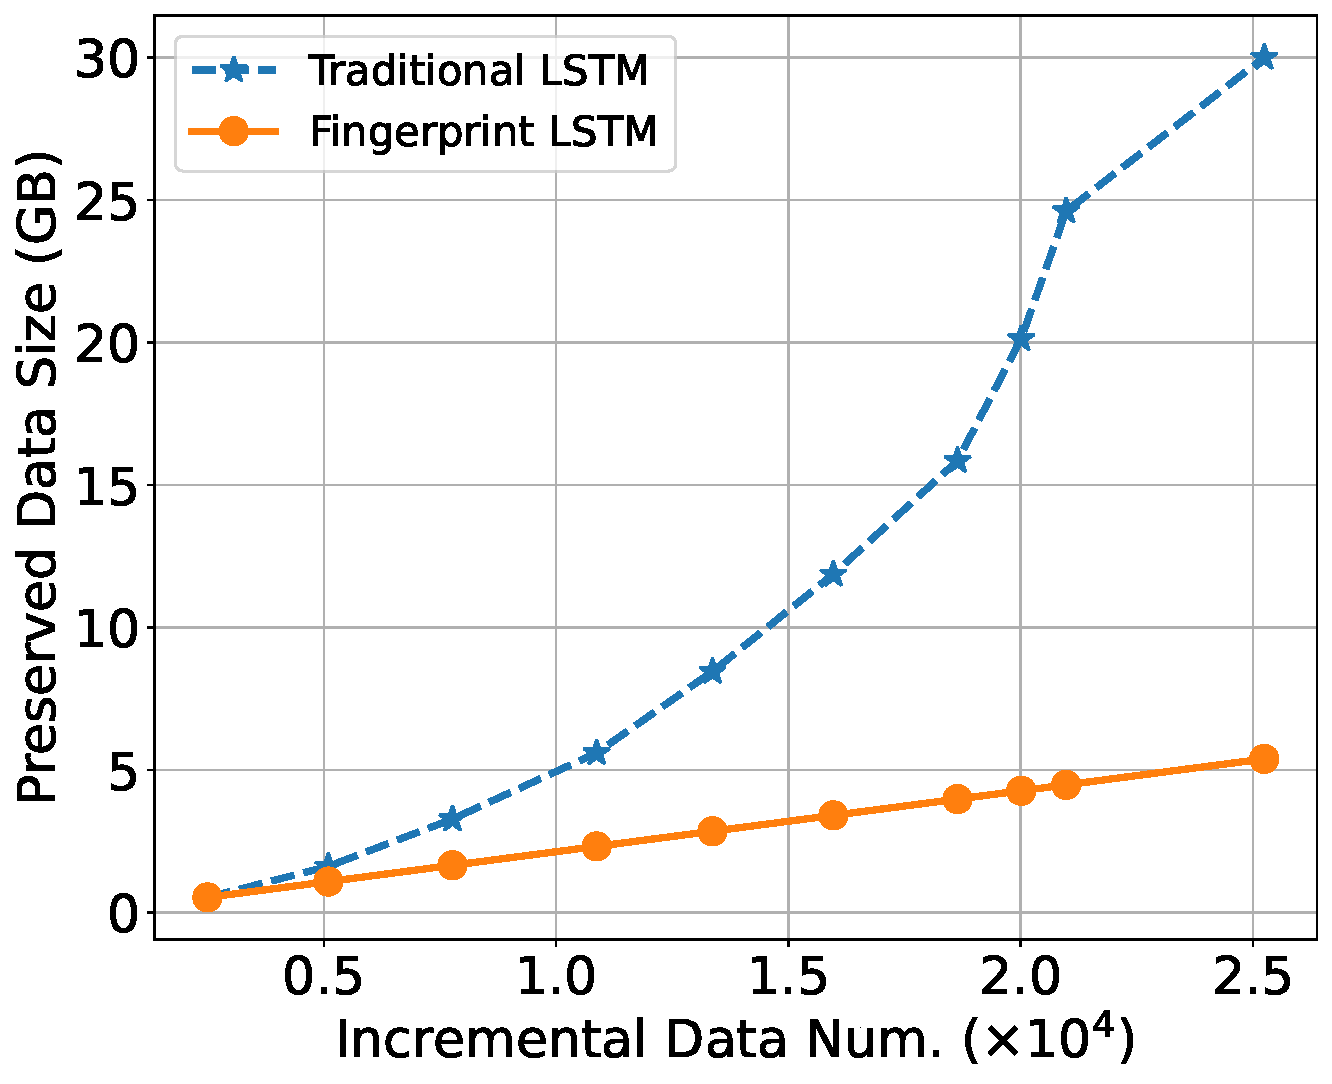
\includegraphics[width=0.47\linewidth]{figs/inc_time_size_cmp_size.pdf}
	}
	\caption{Comparison of training time and size of data needed to be preserved with different numbers of incremental data.}
	\label{fig:inc_time_size}
\end{figure}

\subsubsection{Classification Performance in Different Incremental Scenario}
We verify the classification performance of \sys under different incremental learning scenarios.
We consider three incremental scenarios including the addition of one traffic type, the addition of multiple traffic types at once, and the sequential addition of multiple traffic types.
We first sort the names of traffic types in alphabetical order.
In each incremental scenario, we select the first few traffic types as the incremental traffic types and the remaining traffic types as the initial types. 
Then we train the model to learn new traffic types according to the incremental scenarios. 
Table~\ref{tab:increment_experiment} shows the experiment results. 
In Table~\ref{tab:increment_experiment}, the symbol plus ($+$) means that the corresponding type is added for incremental learning.
The \emph{new} means traffic types newly added during incremental learning and the \emph{old} means traffic types before incremental learning. 
We observe that as long as the trained traffic types are the same (including those gradually added for incremental learning),  the performance of the \sys will be the same. 
This indicates that incremental learning of \sys has the same effect as the training model with full data at once.
In other words, our incremental learning algorithm of \sys does not cause a degradation in classification performance.  

\begin{table}[htbp]
	\centering
	\caption{Classification Performance (F1-Score) Under Different Incremental Learning Scenarios}		
	\label{tab:increment_experiment}
	\begin{tabular}{|c|c|c|c|}
	\hline
	Scenario                                                                                  & Total                   & New                     & Old                     \\ \hline
	+Benign                                                                                   & \textbf{0.9861}                  & 0.9899                  & 0.9855                  \\ 
	+Benign \& Botnet                                                                         & \textbf{0.9861}                  & 0.9886                  & 0.9852                  \\ 
	\multirow{2}{*}{\begin{tabular}[c]{@{}c@{}}+Benign \& Botnet\\ $\rightarrow$+DDoS \& DoS\end{tabular}} & \multirow{2}{*}{\textbf{0.9861}} & \multirow{2}{*}{0.9891} & \multirow{2}{*}{0.9829} \\
	                                                                                          &                         &                         &                         \\ \hline
	\end{tabular}
\end{table}

\subsection{Evaluation of Interpretability}
For the model interpretability of \sys, we first evaluate the global and local interpretability respectively, and then the effectiveness of inter-class distance.
\subsubsection{Effectiveness of Global Feature Ranking}
To examine the effectiveness of features ranked by different methods, we first partition the ranked features into two equal groups, that is, each group has 8 features. 
Then we use features in each group to classify the traffic.
The results are shown in Fig.~\ref{fig:feature_rank_cmp_group}.
We can observe that the first group of \sys has a better F1-Score than the second group.
This indicates that the feature ranking of \sys is effective.
Moreover, we validate the effectiveness of feature ranking by selecting a different number of features according to feature ranking results to perform classification tasks. 
Fig.~\ref{fig:feature_rank_cmp_num_acc}~and~\ref{fig:feature_rank_cmp_num_f1} show the experiment results. 
Compared with other feature ranking methods, our method can achieve higher classification performance with the same number of features. 
This suggests that our feature ranking method can choose the important features of time-series data and is more effective than other feature ranking methods. 
Particularly, using our feature ranking method can achieve classification performance similar to using all features with only half the number of original features. 
Finally, we also compare the time cost of different feature ranking methods and the results are shown in Fig.~\ref{fig:feature_rank_cmp_time}.
We can see that \sys uses the shortest time to rank features while other methods need a longer time to handle or are even impossible to get results in a tolerable time (see a red cross in RFE).
We argue that the efficiency of the feature ranking method is also a part of the interpretable evaluation, which allows users to have quick feedback and a good user experience. 

\begin{figure}[htbp]
	\centering
	\subfloat[]{
		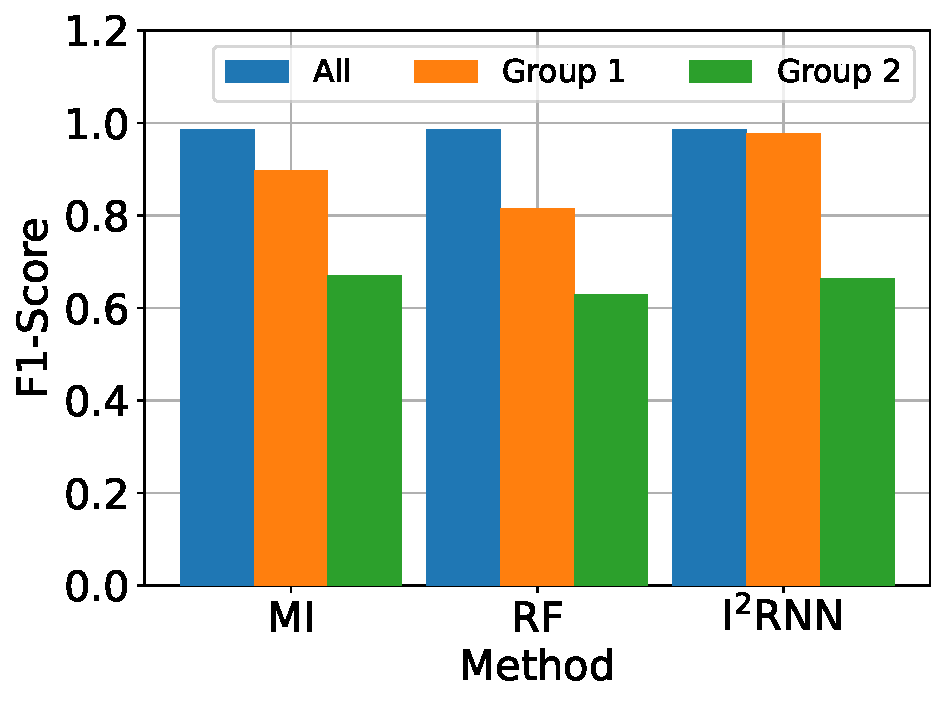
\includegraphics[width=0.47\linewidth]{figs/fea_rank_cmp_group.pdf}
		\label{fig:feature_rank_cmp_group}
	}\hfill
	\subfloat[]{
		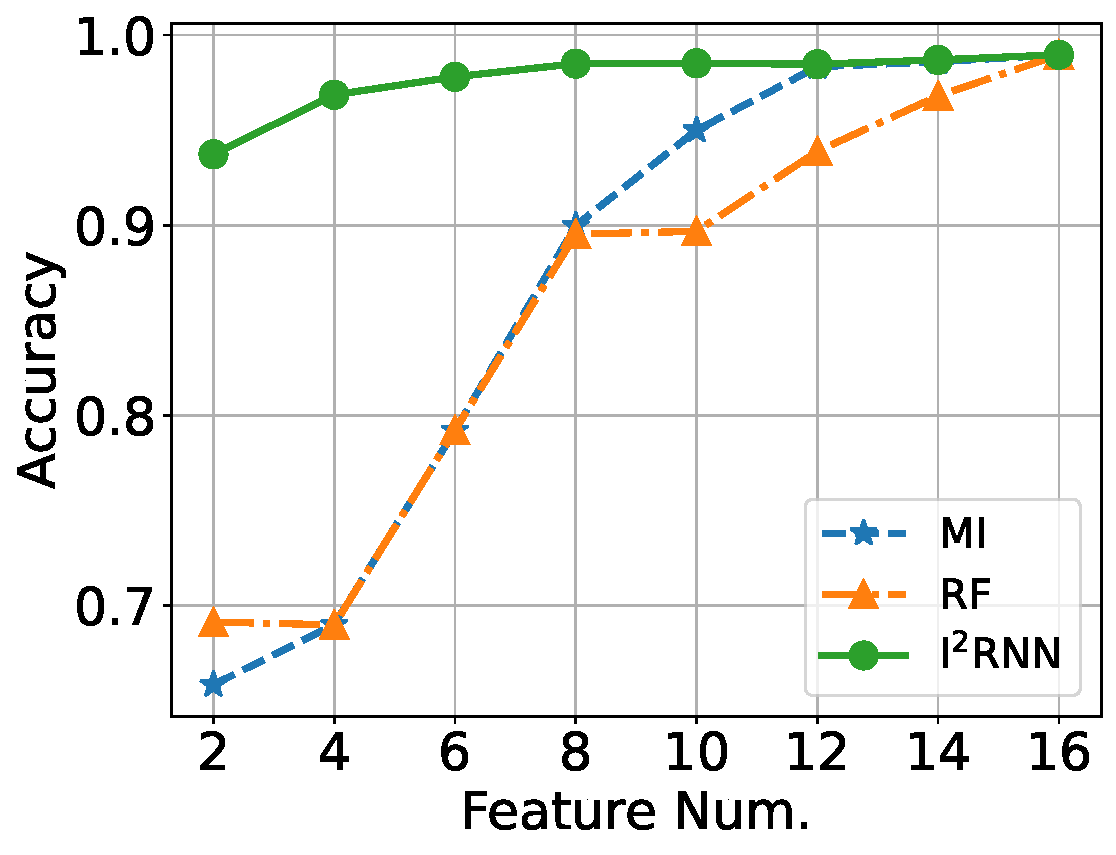
\includegraphics[width=0.47\linewidth]{figs/fea_rank_cmp_num_acc.pdf}
		\label{fig:feature_rank_cmp_num_acc}
	}\\
	\subfloat[]{
		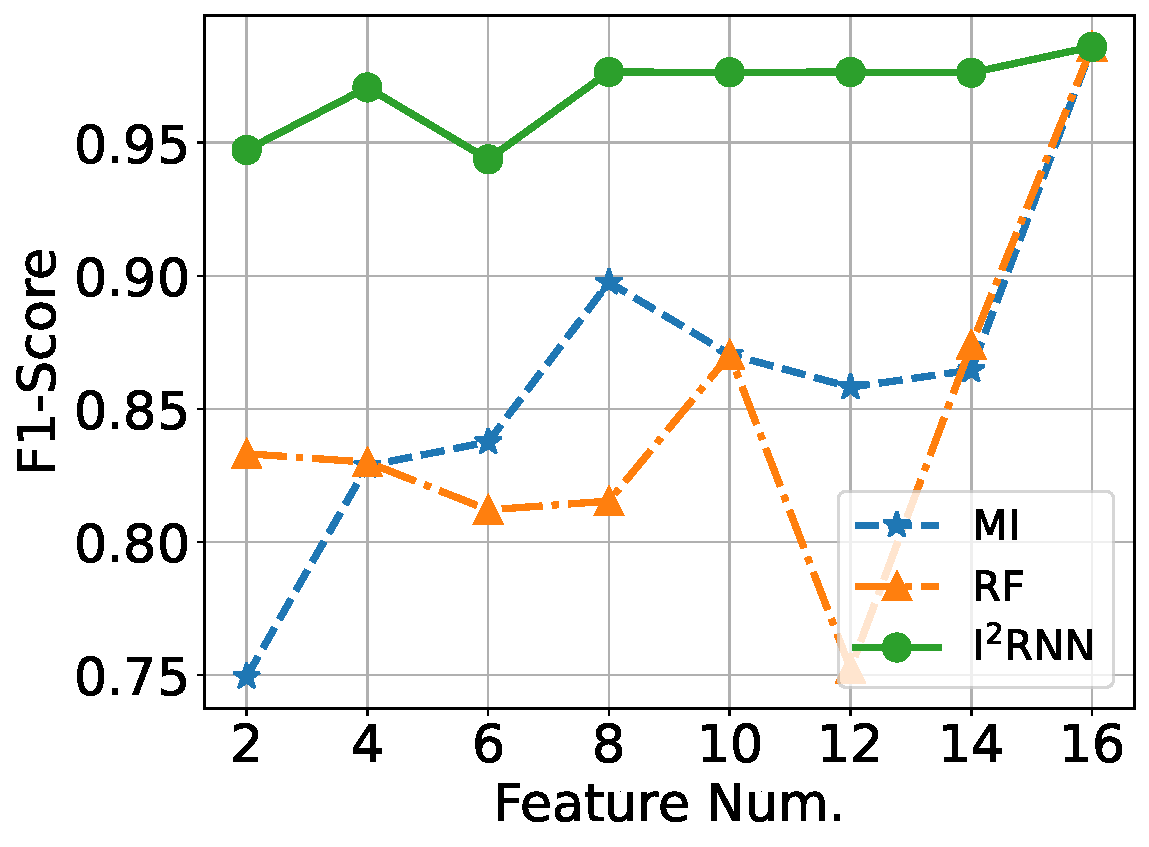
\includegraphics[width=0.47\linewidth]{figs/fea_rank_cmp_num_f1.pdf}
		\label{fig:feature_rank_cmp_num_f1}
	}\hfill
	\subfloat[]{
		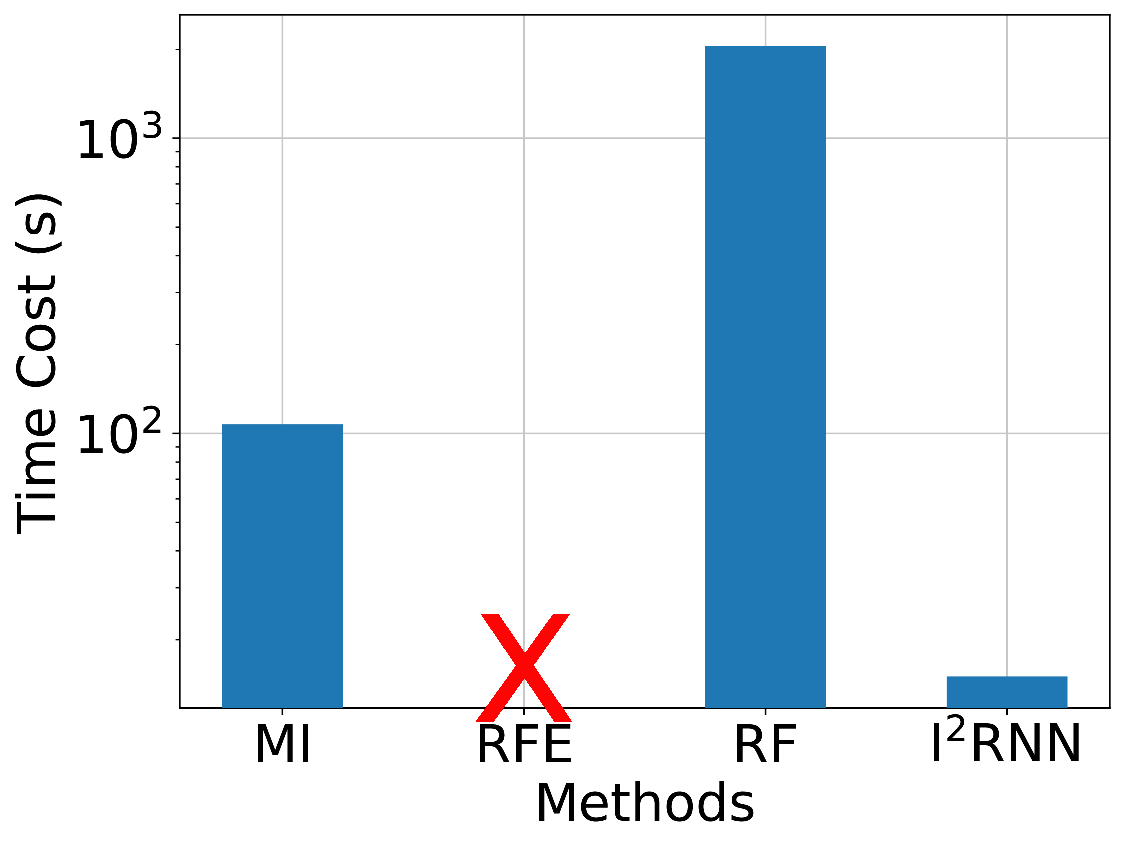
\includegraphics[width=0.47\linewidth]{figs/fea_rank_cmp_time.pdf}
		\label{fig:feature_rank_cmp_time}
	}
	\caption{Experiment results of global model interpretability.}
	\label{fig:experiment_results_interpretability}
\end{figure}

\subsubsection{Performance Comparison of Local Interpretability}
We compare the performance of the local interpretability of \sys with LIME~\cite{lime}, SHAP~\cite{shap}, and feature permutation (PERM)~\cite{altmann2010permutation} in terms of stability, robustness, and effectiveness~\cite{fan2020can}. 
Stability is the fundamental metric of local interpretability. 
The explanation results generated in a critical security system should be stable. 
That is, the feature importance must not be seriously influenced by the slight fluctuation of the model (\eg n\_epochs = 95, n\_epochs = 100, and n\_epochs = 105). 
Robustness is used to measure how similar the explanation results are for similar instances, \ie the feature importance of samples of the same class should be similar, while the feature importance of samples of different classes should be as distinct as possible. 
Effectiveness is the measure of whether the explanation results are important to the decision-making. 
In other words, if the explanation results are really the decision basis for an individual prediction, then after the elimination of such features, the classification result would be changed. 

\begin{figure}[htbp]
	\centering
	\subfloat[Stability]{
		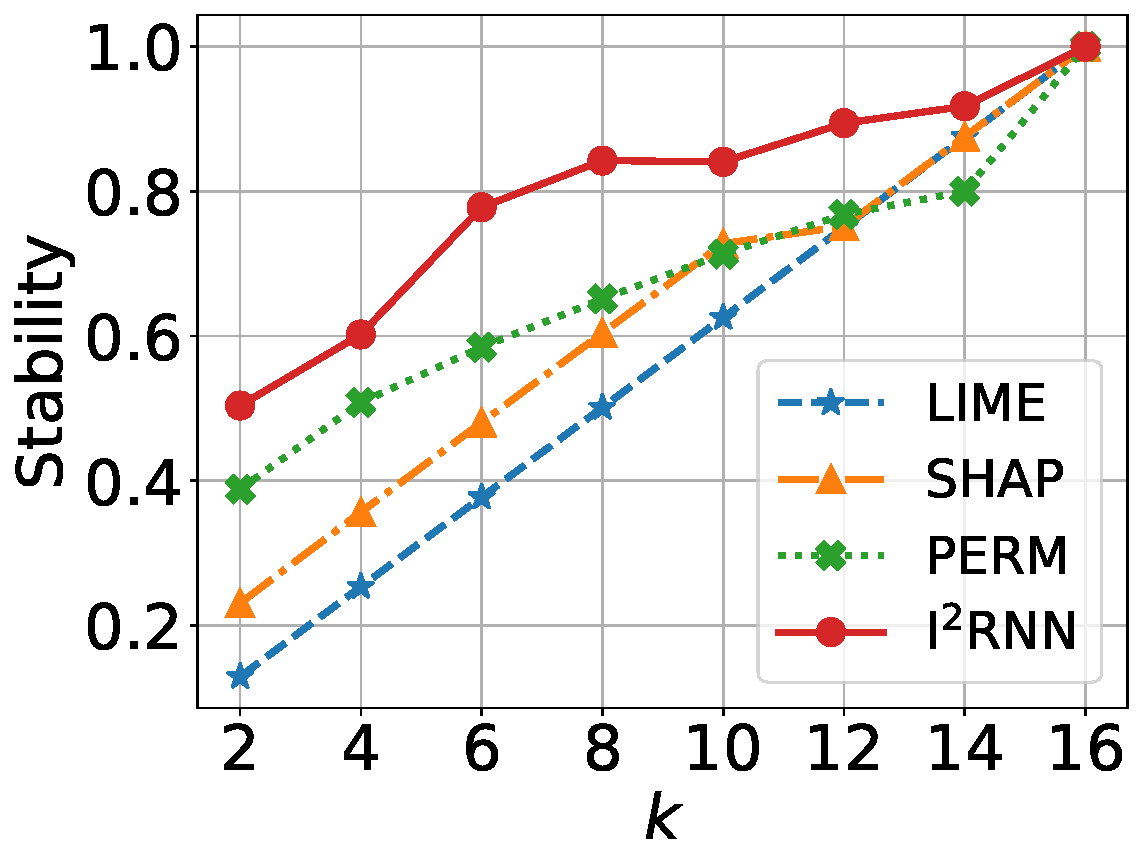
\includegraphics[width=0.47\linewidth]{figs/fea_local_cmp_stability.pdf}
		\label{fig:interpret_stability}
	}\hfill
	\subfloat[Robustness]{
		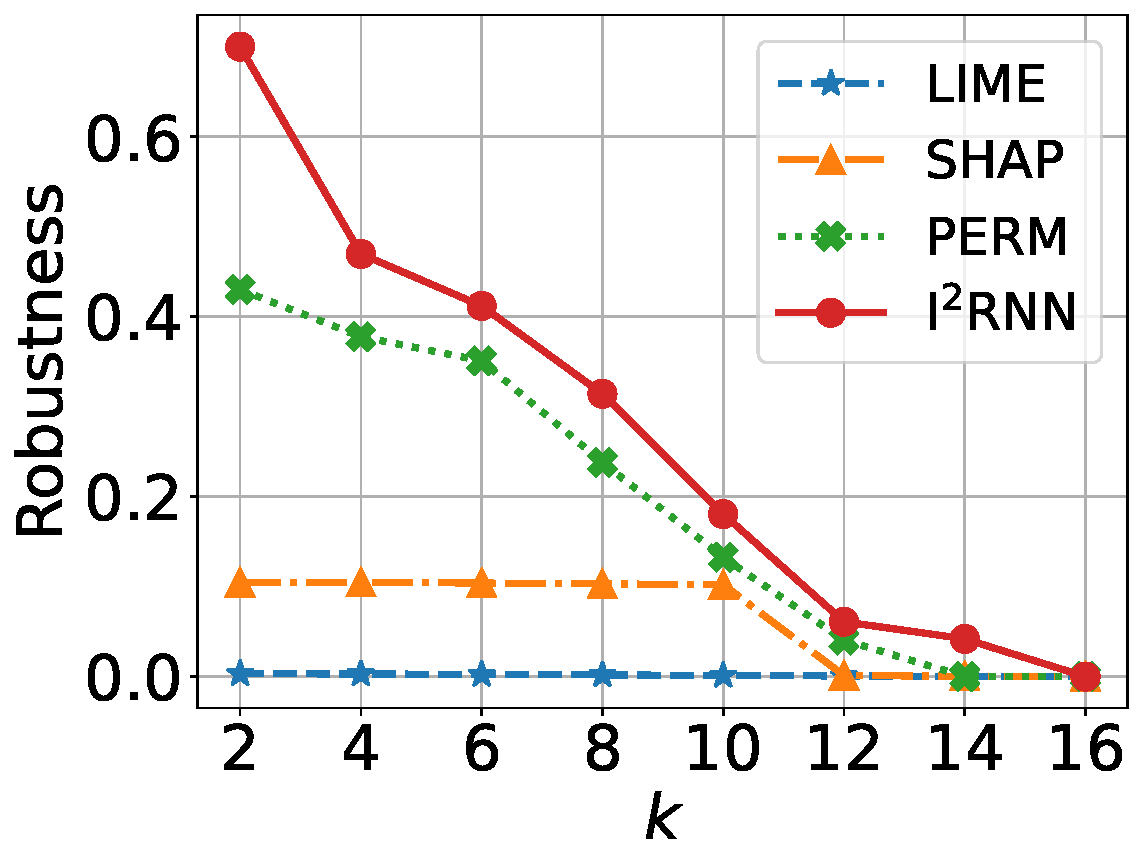
\includegraphics[width=0.47\linewidth]{figs/fea_local_cmp_robustness.pdf}
		\label{fig:interpret_robustness}
	}\hfill
	\subfloat[Effectiveness]{
		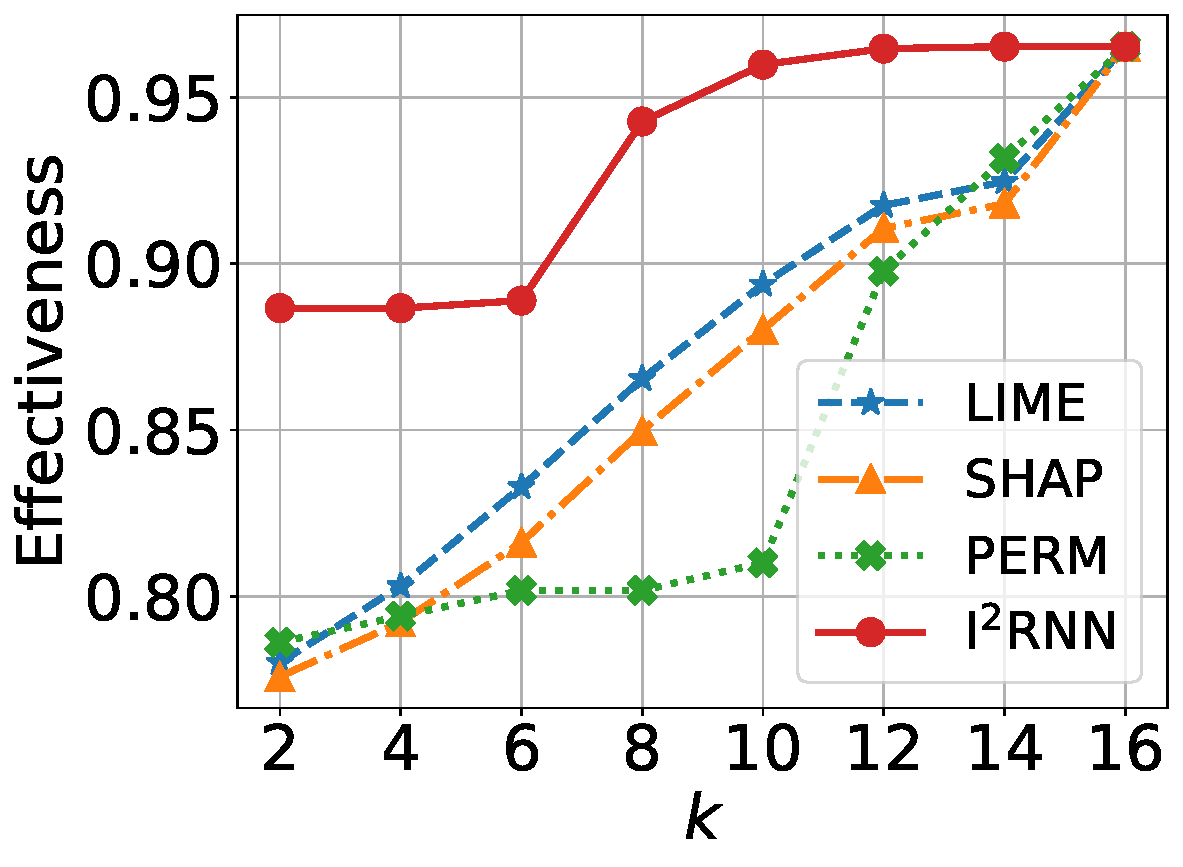
\includegraphics[width=0.47\linewidth]{figs/fea_local_cmp_effectiveness.pdf}
		\label{fig:interpret_effectiveness}
	}\hfill
	\caption{Performance comparison of local interpretability.}
	\label{fig:experiment_results_local_interpretability}
\end{figure}

Fig.~\ref{fig:experiment_results_local_interpretability} illustrates the performance comparison of local interpretability in terms of stability, robustness, and effectiveness under different top-$k$ features. 
From the figure, we can observe that:
\begin{itemize}
\item The \sys shows the best stability, robustness, and effectiveness compared to other methods under different top-$k$ features. 
\item The ranking of the four local interpretability approaches in term of the stability metric is \sys $>$ PERM $>$ SHAP $>$ LIME. The stability of \sys is above 0.8 when $k \ge 6$, indicating that explanation features hardly change when slightly modifying the model. 
\item The ranking of the four local interpretability approaches in term of the robustness metric is \sys $>$ PERM $>$ SHAP $>$ LIME. With the increase of $k$, the robustness of the four methods decreases. For SHAP and LIME, their robustness scores are lower than 0.2, and they hardly change under various $k$ values. The robustness of PERM is less than 0.5. These indicate that PERM, SHAP, and LIME cannot capture the core differences between traffic types especially when $k$ is small.
\item The ranking of the four local interpretability approaches in term of the effectiveness metric is \sys $>$ LIME $\ge$ SHAP $>$ PERM. The effectiveness of LIME and SHAP is very similar. For \sys, the effectiveness starts to be stable when $k > 8$. This indicates important features of \sys are in the top half of the ranked features, which results in little change of predicted label with higher $k$ values.
\end{itemize}

\subsubsection{Effectiveness of Inter-Class Distance}\label{sec:group}
To validate whether inter-class distance effectively characterizes the similarity between traffic types, we group traffic types with close distance as an individual traffic type. 
As depicted in Fig.~\ref{fig:traffic_distance}, Botnet and Brute Force are the closest in all features and thus we group them into an individual type. 
We also group DDoS and DoS which are close in all features. 
For a fair comparison (i.e., taking out the factor of category reduction), we also group traffic types with large distances. 
We group Port Scan and SSH Patator which are the farthest types in all features. 
Benign and DDoS are also grouped as an experiment for large distances. 
The results are shown in Table~\ref{tab:group_experiment}. 
We can observe that the performance is improved if we group traffic types that have small inter-class distances (i.e., they are close in some dimensions or in all features), while the performance significantly decreases if we group traffic types with large distances. 
These results indicate that our inter-class distance is rational, which captures the relationships between traffic types. 

\begin{table}[htbp]
	\centering
	\caption{Experiment Results of Different Grouping Strategies}		
	\label{tab:group_experiment}
	    \begin{tabular}{|c|c|c|c|}
	    \hline
	    Grouping Strategy & Distance & AC (\%) & F1 (\%) \\
	    \hline
	    \textbf{Botnet} \& \textbf{Brute Force} & \textbf{0.65} & \textbf{99.95} & \textbf{98.90} \\
	    \textbf{DDoS} \& \textbf{DoS} & \textbf{1.28} & \textbf{99.64} & \textbf{98.81} \\
	    \hline
	    Benign \& DDoS & 2.67 & 91.24 & 85.31 \\
           Port Scan \& SSH Patator & 7.49 & 79.71 & 80.84 \\
	    \hline
	    \end{tabular}
\end{table}
\section{Discussion}
\label{sec:Discussion}
\sys with fingerprint learning has shown a great advantage in encrypted traffic classification. 
It can be deployed as a model capable of efficient incremental learning to cope with the ever-increasing types of traffic in the real world. 
The global level feature ranking and selection help eliminate unnecessary features and alleviate the computational overhead. 
Moreover, researchers and users can understand the deep insights for the model's predictions from the local feature interpretation with high stability, robustness, and effectiveness. 
Besides, \sys profiles the differences and relations between traffic types with the inter-class distance portrait. 
Users can group similar traffic types to improve classification performance in practice. 
Below, we discuss the identification of new traffic types, model scalability, and limitations. 

\textbf{Where do the new traffic types come from?} Though \sys focuses on coping with the incremental learning scenario, with the ability to incrementally learn new types without accessing past data and retraining the model, it is natural to think about where the new traffic types come from. 
Currently, the newly labeled data for updating the model are manually proposed by the same party who uses the model for detection.
We can obtain new application types by collecting relevant information in the application markets such as App Store and Google Play.
New types of attacks may be reported by researchers after analyzing system logs and traffic data.
Some arts~\cite{shen2019encrypted,zhang2020autonomous} also propose open-set recognition for encrypted traffic classification, which focus on automatically recognizing and labeling new traffic types.
\sys could leverage these methods to improve the identification of new traffic types and build a more automatic incremental learning process.

\textbf{What is the scalability of the model?} As the number of fingerprint modules increases, the scalability of the \sys may become a concern for users.
Here we clarify the scalability of \sys in terms of space and time. 
In terms of space, each fingerprint module is lightweight and does not take up too much disk space.
For example, the number of parameters of each fingerprint module trained on ISCXVPN2016 is only 5334. 
The size of the hard disk space occupied by each fingerprint module is only 23.17 KB. 
Therefore, even if the fingerprint module continues to increase, there will be no obvious scalability problem in space. 
In terms of time, since each fingerprint module is independent, the network traffic data can be simultaneously fed into each fingerprint module for parallel computation. 
Therefore, the computing capacity practically depends on the maximum number of parallel threads the CPU allowed. 
Furthermore, this computational process can be extended to distributed computing clusters using the idea of MapReduce~\cite{dean2008mapreduce}.
Fingerprint modules can be deployed on multiple computing nodes.
When new traffic data arrives, each computing node can calculate the loss for the input traffic in parallel.
After waiting for all computing nodes to complete the calculation, we can aggregate all losses and give the final prediction results by comparing the outputs of each fingerprint module. 
Therefore, even if the fingerprint module keeps increasing, the model will also maintain good scalability in time.

\textbf{Limitations and Future Work.} There are still two limitations of \sys. 
The first limitation is that the fingerprint may be outdated over time as the behavior of the corresponding traffic type may vary at different times.
Future work can develop some systematic strategies to periodically update the fingerprint modules in \sys. 
The second limitation is that hyper-parameters of \sys are configured empirically. 
Future work can investigate the sensitivity of hyper-parameters, and provide brief guidelines about how to configure them.




\section{Conclusions}
\label{sec:Conclusions}
In this paper,  we have presented \sys, an incremental and interpretable recurrent neural network model for encrypted traffic classification. 
The \sys learns fingerprints from the raw session sequences, which has local robustness. 
The \sys considers an incremental learning scenario. % and is designed as an incremental model. 
It only needs to train an additional set of parameters for the newly added traffic type rather than retraining the whole model.  
Moreover, the \sys is an interpretable model, which provides the feature attribution globally and locally. 
It can also depict the similarity between traffic types through inter-class distance.
The evaluation results on two public datasets demonstrate that our \sys can achieve remarkable performance in terms of encrypted traffic classification, incremental learning, and model interpretability. 
In performance comparison with well-known local interpretability methods, our \sys exhibits excellent stability, robustness, and effectiveness in the interpretation of network traffic data. 
In future work,  we plan to investigate effective techniques for identifying new types of traffic automatically and updating the learned fingerprints to keep pace with the time evolution of traffic.
\section*{Acknowledgements}
This work was supported in part by National Natural Science Foundation of China (62227805, 62072398), by SUTD-ZJU IDEA Grant for visiting professors (SUTD-ZJUVP201901), by National Key R\&D Program of China (2020AAA0107700),  by Alibaba-Zhejiang University Joint Institute of Frontier Technologies, by Zhejiang Key R\&D Plan (2021C01116), by Leading Innovative and Entrepreneur Team Introduction Program of Zhejiang (2018R01005), by Research Institute of Cyberspace Governance in Zhejiang University, by National Key Laboratory of Science and Technology on Information System Security (6142111210301), by State Key Laboratory of Mathematical Engineering and Advanced Computing, and by Key Laboratory of Cyberspace Situation Awareness of Henan Province (HNTS2022001).

\bibliographystyle{IEEEtran}
\bibliography{IEEEabrv, ref}

% biography section
% 
% If you have an EPS/PDF photo (graphicx package needed) extra braces are
% needed around the contents of the optional argument to biography to prevent
% the LaTeX parser from getting confused when it sees the complicated
% \includegraphics command within an optional argument. (You could create
% your own custom macro containing the \includegraphics command to make things
% simpler here.)
%\begin{IEEEbiography}[{\includegraphics[width=1in,height=1.25in,clip,keepaspectratio]{mshell}}]{Michael Shell}
% or if you just want to reserve a space for a photo:

%\begin{IEEEbiography}{Michael Shell}
%Biography text here.
%\end{IEEEbiography}

% if you will not have a photo at all:
%\begin{IEEEbiographynophoto}{John Doe}
%Biography text here.
%\end{IEEEbiographynophoto}

% insert where needed to balance the two columns on the last page with
% biographies
\newpage

%\begin{IEEEbiographynophoto}{Jane Doe}
%Biography text here.
%\end{IEEEbiographynophoto}

% You can push biographies down or up by placing
% a \vfill before or after them. The appropriate
% use of \vfill depends on what kind of text is
% on the last page and whether or not the columns
% are being equalized.

\begin{IEEEbiography}
[{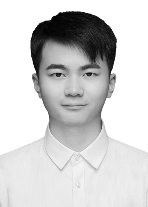
\includegraphics[width=1in,height=1.25in,clip,keepaspectratio]{./figs/szx.pdf}}]
{Zhuoxue Song} received the B.S. degree in computer science and technology from Hangzhou Dianzi University, in 2021. 
He is currently working toward the M.S. degree in the security of cyberspace at Zhejiang University. 
His main research interests include encrypted traffic classification and intrusion detection.
\end{IEEEbiography}

\begin{IEEEbiography}
[{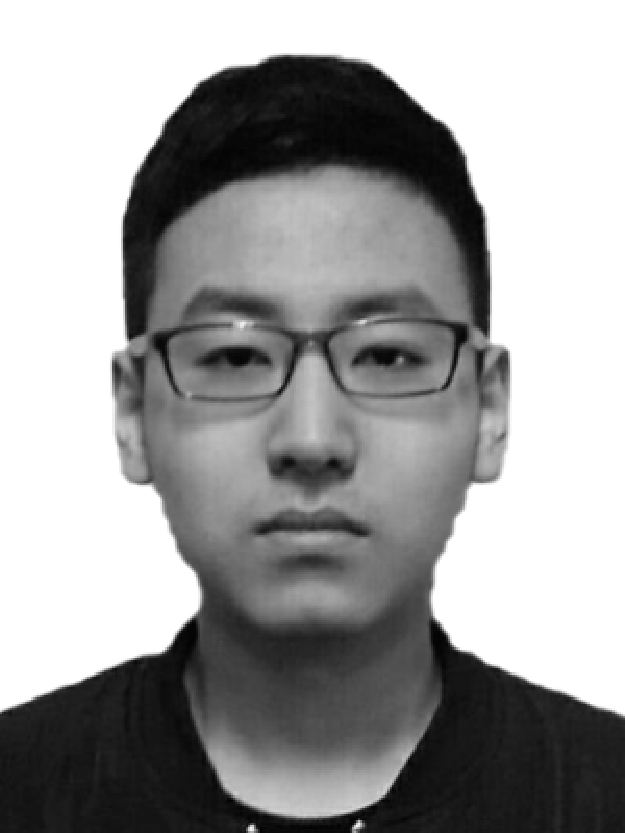
\includegraphics[width=1in,height=1.25in,clip,keepaspectratio]{./figs/zzm.pdf}}]
{Ziming Zhao} received the B.S. degree in computer science and technology from Shijiazhuang Tiedao University, in 2019.
He is currently working toward the Ph.D. degree in the security of cyberspace at Zhejiang University. 
His main research interests include network security and intrusion detection.
\end{IEEEbiography}

\begin{IEEEbiography}
[{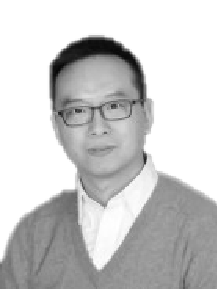
\includegraphics[width=1in,height=1.25in,clip,keepaspectratio]{./figs/zf.pdf}}]
{Fan Zhang} (Member,~IEEE) received the Ph.D. degree from the Department of Computer Science and Engineering, University of Connecticut, Mansfield, CT, USA, in 2011.
He is currently a Full Professor with the College of Computer Science and Technology, Zhejiang University, Hangzhou, China, and also with the Alibaba–Zhejiang University Joint Institute of Frontier Technologies, Hangzhou. 
His research interests include system security, hardware security, network security, and cryptography.
\end{IEEEbiography}

\begin{IEEEbiography}
[{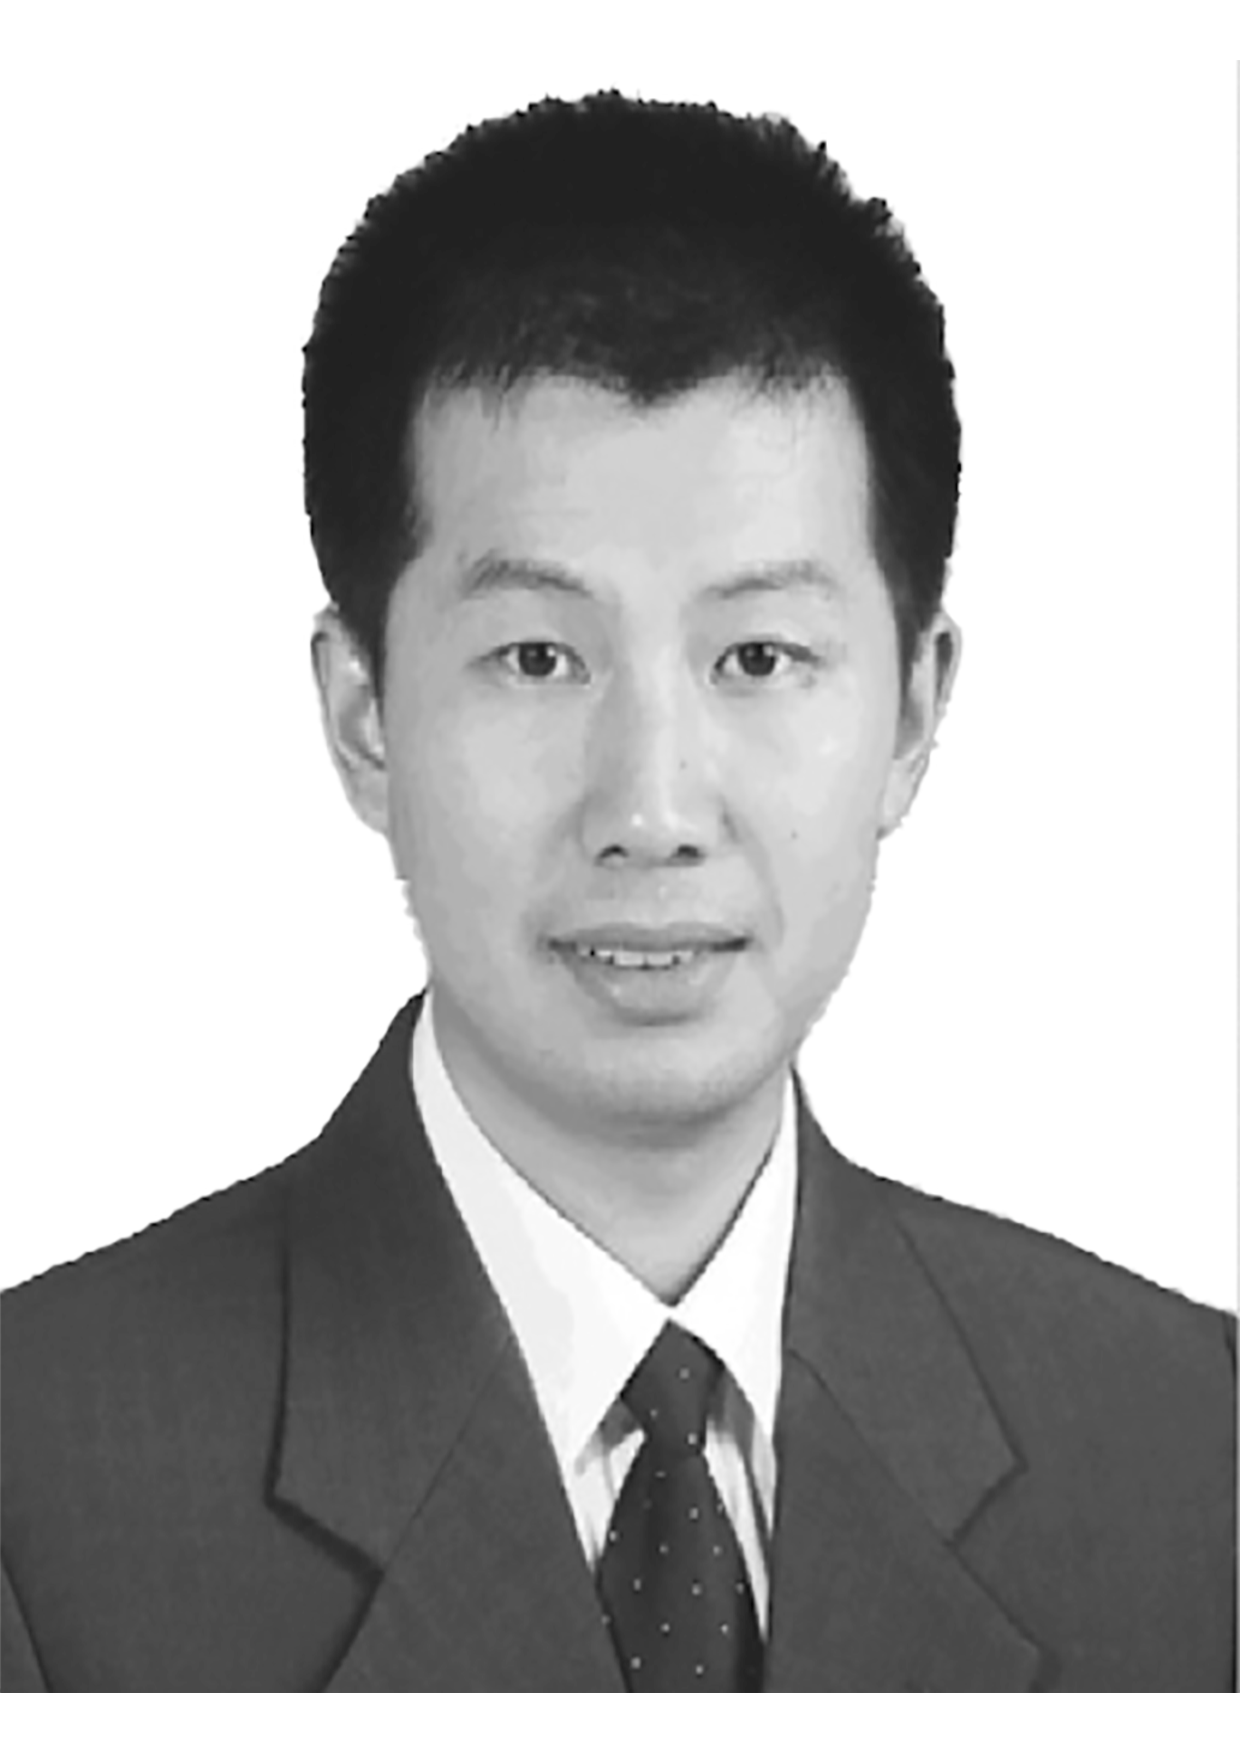
\includegraphics[width=1in,height=1.25in,clip,keepaspectratio]{./figs/xg.pdf}}]
{Gang Xiong} is currently a Full Professor and Ph.D. Supervisor with the Institute of Information Engineering, Chinese Academy of Sciences, China. He has authored more than 60 papers in refereed journals and conference proceedings. His research interests include network and information security. He is a member of the 3rd Communication Security Technical Committee of China Institute of Communications.
\end{IEEEbiography}
\vfill
\newpage
\begin{IEEEbiography}
[{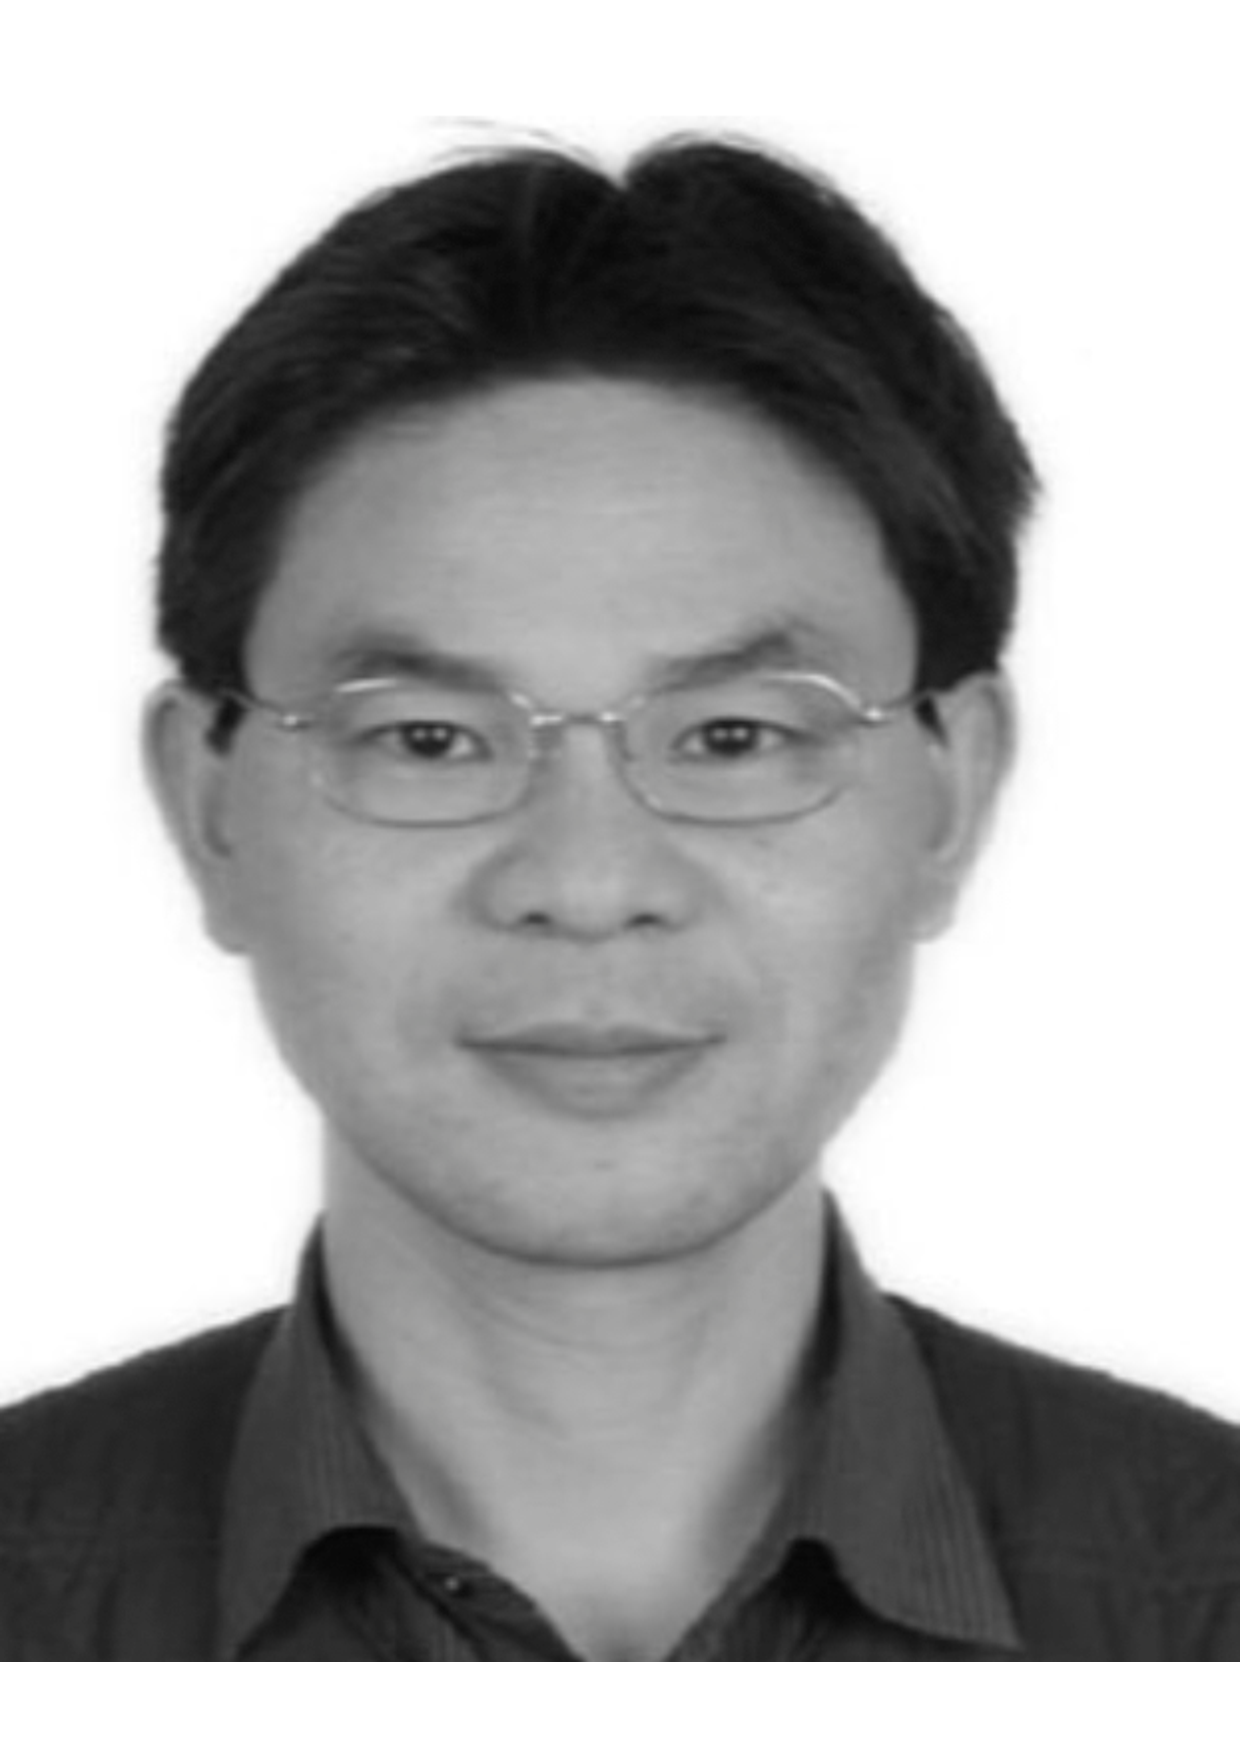
\includegraphics[width=1in,height=1.25in,clip,keepaspectratio]{./figs/cg.pdf}}]
{Guang Cheng} (Member,~IEEE) received the B.S. degree in traffic engineering from Southeast University, Nanjing, China, in 1994, the M.S. degree in computer application from the Hefei University of Technology, Hefei, China, in 2000, and the Ph.D. degree in computer network from Southeast University, in 2003.
He is currently a Full Professor with the School of Cyber Science and Engineering, Southeast University. He has authored or coauthored seven monographs and more than 100
technical papers, including top journals and top conferences. 
His research interests include network security, network measurement, and traffic behavior analysis.
\end{IEEEbiography}

\begin{IEEEbiography}
[{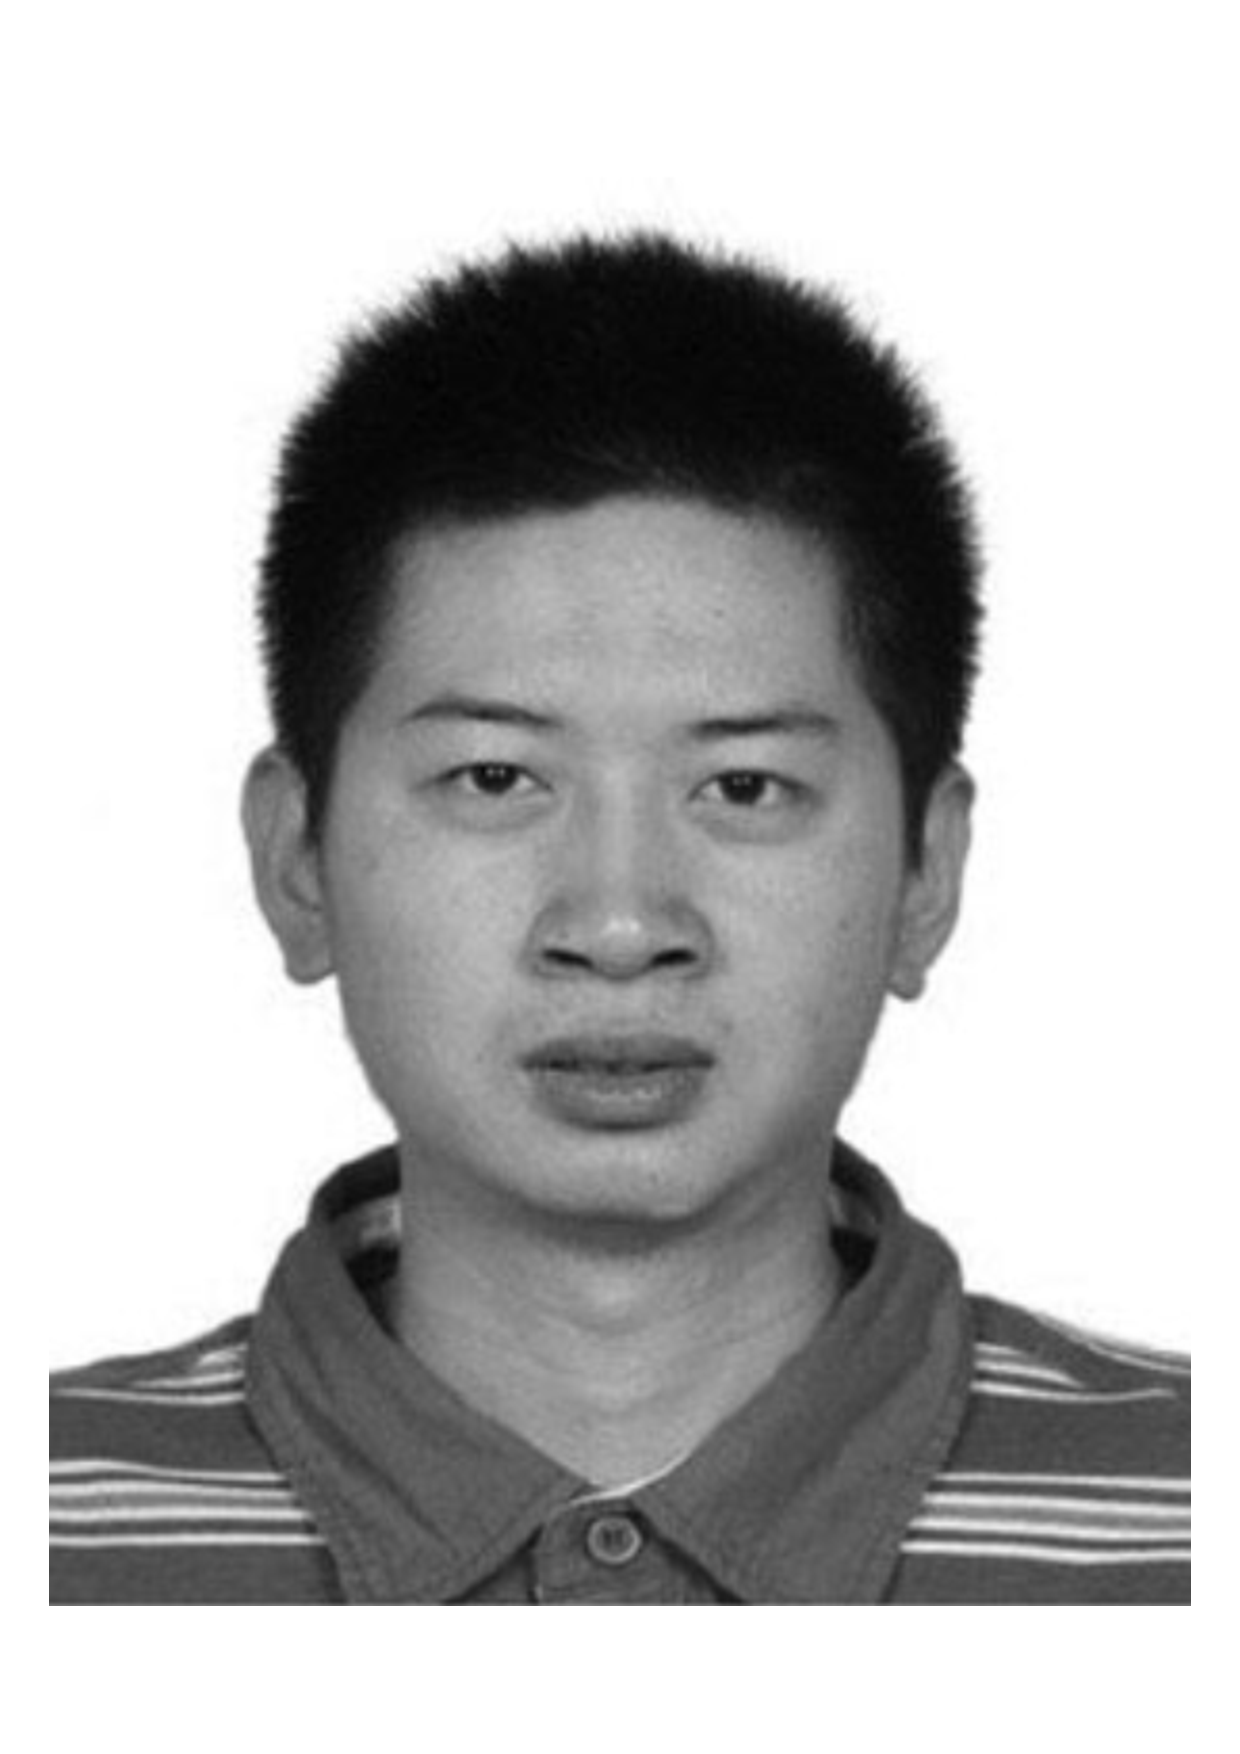
\includegraphics[width=1in,height=1.25in,clip,keepaspectratio]{./figs/zxj.pdf}}]
{Xinjie Zhao} received the B.S., M.S., and Ph.D. degrees from Ordnance Engineering College, Shijiazhuang, China, in 2006, 2009, and 2012, respectively.
He is currently with the College of Computer Science and Technology, Zhejiang University, Hangzhou, China. His main research interests include side channel analysis, fault analysis, and combined analysis in cryptography.
Dr. Zhao won the best paper award in COSADE 2012.
\end{IEEEbiography}

\begin{IEEEbiography}
[{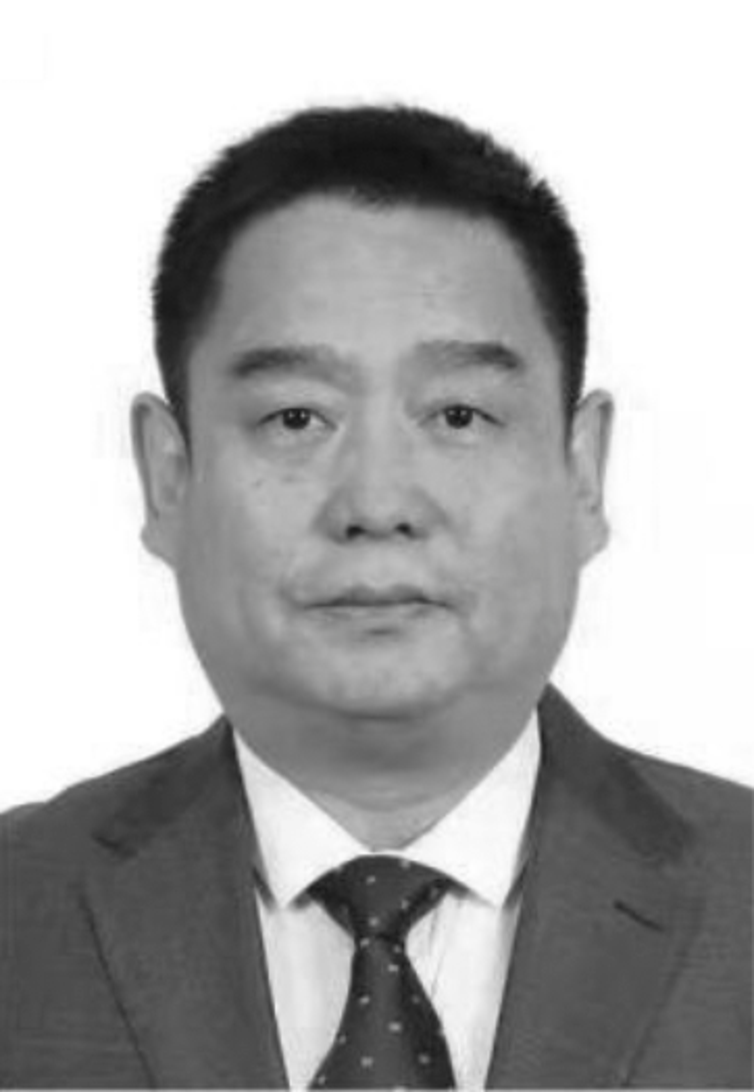
\includegraphics[width=1in,height=1.25in,clip,keepaspectratio]{./figs/gsz.pdf}}]
{Shize Guo} received the B.S. and M.S. degrees from Ordnance Engineering College, China, in 1988 and 1991, respectively, and the Ph.D. degree from the Harbin Institute of Technology, in 1994. He is currently with the College of Computer Science and Technology, Zhejiang University, Hangzhou, China. His main research interests include information technology and information security.
\end{IEEEbiography}

\vfill

\vfill

% Can be used to pull up biographies so that the bottom of the last one
% is flush with the other column.
%\enlargethispage{-5in}

\end{document}


